\documentclass[letterpaper,10pt]{book}
% Change to 10 pt
\usepackage{pdfpages}
\usepackage{morewrites}			% to counteract the no write space problem
\setcounter{tocdepth}{6}

\usepackage[framemethod=TikZ]{mdframed}

\usepackage{fancyhdr}

\usepackage{paralist}
\usepackage{amsmath}
\usepackage{amsfonts}
\usepackage{amssymb}
\usepackage{graphicx}

\usepackage{datetime}
%\usepackage{ulem}

%\usepackage[nottoc]{toobibind}

\usepackage[inline]{enumitem}

% Outer margin at 2.50 is exacty correct to fit the ``corruption alert'' tables
\usepackage[inner=1.0in, outer=2.50in, top=2.54cm,bottom=2.54cm, marginparwidth=2.25in]{geometry}

\usepackage{marginnote}
\usepackage{longtable}
\usepackage{booktabs}
\usepackage{xcolor}

\usepackage{soul}

%%%%%%%%%%%%
\definecolor{ForestGreen}{rgb}{0.00,0.29,0.098}
%%%%%%%%%%%%

\usepackage{marginnote}

\usepackage{imakeidx} 
\usepackage[
	backref=true,
	style=numeric,
%	citestyle=numeric,
	backend=bibtex
	]{biblatex}
\usepackage[driverfallback=hypertex,colorlinks=True]{hyperref}
\usepackage{cleveref}

\makeindex[name=scripture,columnsep=20pt, columnseprule=True,columns=3, title=Scripture References]
\makeindex[name=speaker,columnsep=20pt, columnseprule=True,,columns=2, title=Sermon Creator]
\makeindex[name=series,columnsep=20pt, columnseprule=True,,columns=2, title=Sermon Series]
\makeindex[name=date,columnsep=20pt, columnseprule=True,columns=2, title=Sermon Date]
\makeindex[name=event,columnsep=20pt, columnseprule=True,columns=2, title=Event]
\makeindex[name=topic,columnsep=20pt, columnseprule=True,columns=2, title=Topic]
\makeindex[name=AWIP,columnsep=20pt, columnseprule=True,columns=3, title=All Words in Passage]
\makeindex[name=NWIV,columnsep=20pt, columnseprule=True,columns=3, title=Number of Words in Verse]
\makeindex[name=PNIP,columnsep=20pt, columnseprule=True,columns=3, title=Proper Names in Passage]
\makeindex[name=PEIP,columnsep=20pt, columnseprule=True,columns=2, title=Prophetic Events in Passage]
\makeindex[name=TWPAQ,columnsep=20pt, columnseprule=True,columns=1, title=13-Word Phrases and Quotes]
\makeindex[name=PFTTIS,columnsep=20pt, columnseprule=False,columns=3, title=Phrases found 13 times in scripture]
\makeindex[name=WFTTIS,columnsep=20pt, columnseprule=False,columns=3, title=Words found 13 times in scripture]
\makeindex[name=WFITV,columnsep=20pt, columnseprule=False,columns=3, title=Words found in exactly 13 verses]
\makeindex[name=EVENTS,columnsep=20pt, columnseprule=False,columns=2, title=Sermon Log by Place]
\makeindex[name=QUESTIONS,columnsep=20pt, columnseprule=False,columns=2, title=Bible Questions]
\makeindex[name=DOCTRINES,columnsep=20pt, columnseprule=False,columns=2, title=Doctrines]
\makeindex[name=SONGS,columnsep=20pt, columnseprule=False,columns=1, title=Songs]
\makeindex[name=LOCATION,columnsep=20pt, columnseprule=False,columns= 2, title=Location]
\makeindex[name=FACEBOOK,columnsep=20pt, columnseprule=False,columns=2, title=Facebook]
\makeindex[name=DEVOTIONAL,columnsep=20pt, columnseprule=False,columns=2, title=Devotional Items]
%%%%%%%%%%%%%%%%% EXTRA COLORS
\definecolor{champagne}{rgb}{0.97,0.91,0.81}
\definecolor{bone}{rgb}{0.89,0.85,0.79}
\pagestyle{fancy}
\fancyhf{}
\fancyhead[LE,RO]{\today}
\fancyhead[RE,LO]{Daily Bible Reading}
\fancyhead[CE,CO]{-page \thepage  - }

\fancyfoot[CO,CE]{\leftmark}
%\fancyfoot[LE,RO]{CSCE 692, HW1}

\title{DBR\\
Daily \\ Reads}
\author{Keith Anthony \\
\today }
%+/ffffff +   \pagenumbering{gobble}
\bibliography{Bibliographies/All20220122}

\setlength{\fboxsep}{1.0pt}

\usepackage[utf8]{inputenc}
\usepackage{tikz}

\begin{document}
%%%%%%%%%%%% Tile Page

\begin{titlepage}

\begin{flushright}
\rightskip=-2.5cm
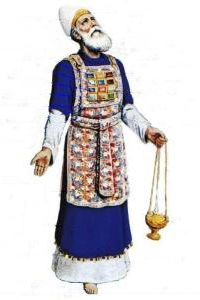
\includegraphics[width=50mm,scale=1.5]{Extras/Melchisedec.jpg}
\vspace{0.4in}  % Create a title for the document and write it in bold font
\LARGE{\textbf{\date}} % Again, do a line break
\linebreak 
% Create a subtitle \large{with Outlines, Statistics, Cross References, and Notes}
\vspace{0.5in}
\begin{flushleft}
\LARGE{Day \#72: Monday, 14 March 2022 PLAIN  \\}\vspace{0.25in}
\LARGE{Judges 1-3 Psalm 73 Proverb 14}
\end{flushleft}
\vspace{0.6in}
\bigskip

\normalsize{Xenia, Oh.\\}
\normalsize{created: \today}
\vspace{1.3in}

\end{flushright}
\end{titlepage}

\newpage 
\tableofcontents\hypertarget{TOC}{}
\listoffigures
\listoftables

\hyphenation{A-bim-e-lech bre-thren E-phra-im  Gib-e-o-nites Jer-u-sa-lem through-out Phil-i-stines The-o-phil-us Am-a-le-kites ven-geance Mesh-el-e-mi-ah onan-ism Phar-a-oh thoughts grev-ous-ness Hach-a-liah adul-ter-er Shad-rach}

%%%%%%%%%%%%%%%%% EXTRA COLORS
%%%%%%%%%%%%%%%%% EXTRA COLORS
%%%%%%%%%%%%%%%%% EXTRA COLORS
\definecolor{champagne}{rgb}{0.97,0.91,0.81}
\definecolor{bone}{rgb}{0.89,0.85,0.79}

\definecolor{ForestGreen}{rgb}{0.00,0.29,0.098}
\definecolor{GIVING}{cmyk}{1,0.0,0.72,.1}

\definecolor{MLPE}{cmyk}{1,1,0,.45}
\definecolor{SOCCER}{cmyk}{.77, 0, .42, .49}
\definecolor{PAYBILL}{cmyk}{0,0.83,0.76,0.07}
\definecolor{SERMON}{cmyk}{.14,.9,0,.30} % aka seance \href{http://www.flatuicolorpicker.com/purple-cmyk-color-model/}{seance}
\definecolor{BIBLE}{cmyk}{0,.17,.74,.17}
\definecolor{WORKBLUE}{cmyk}{1, .5, 0, .6}
\definecolor{myOrange}{cmyk}{0, .4, .98, .03}
\definecolor{myTan}{cmyk}{0.0,.07,.17,.10}
\definecolor{myRed}{cmyk}{0,1,1,0}
\definecolor{myWhite}{cmyk}{0,0,0,0}
\definecolor{BLUESoD}{cmyk}{.97,.84,0,.04}
\definecolor{WHITE}{cmyk}{0,0,0,0}
\definecolor{OLDGOLD}{cmyk}{0.05,0.3,1.00,0}
\definecolor{CASTLETON}{cmyk}{1,0,0.31,0.66}
\definecolor{cadmiumgreen}{rgb}{0.0, 0.42, 0.24}
\definecolor{jungle}{rgb}{0.203,0.4882,0.1718}
\definecolor{MYGOLD}{rgb}{1,.84,0}

\definecolor{MYLIGHTGRAY}{rgb}{.85,.85,.85}

\definecolor{codegreen}{rgb}{0,0.6,0}
\definecolor{codegray}{rgb}{0.5,0.5,0.5}
\definecolor{codepurple}{rgb}{0.58,0,0.82}
\definecolor{backcolour}{rgb}{0.95,0.95,0.92}


\mdfdefinestyle{MyFrame}{%
    linecolor=blue,
    outerlinewidth=2pt,
    roundcorner=5pt,
    innertopmargin=\baselineskip,
    innerbottommargin=\baselineskip,
    innerrightmargin=10pt,
    innerleftmargin=10pt,
    backgroundcolor=gray!25!white}


\mdfdefinestyle{MyFrame2}{%
    linecolor=black,
    outerlinewidth=2pt,
    roundcorner=5pt,
    innertopmargin=\baselineskip,
    innerbottommargin=\baselineskip,
    innerrightmargin=10pt,
    innerleftmargin=10pt,
    backgroundcolor=yellow!25!white}


%%%%%
%% for PFTTIS list
%%%%%

%%% And Joseph said unto
\index[PFTTIS]{And Joseph said unto!Genesis!Gen 40:008}
\index[PFTTIS]{And Joseph said unto!Genesis!Gen 40:012}
\index[PFTTIS]{And Joseph said unto!Genesis!Gen 41:025}
\index[PFTTIS]{And Joseph said unto!Genesis!Gen 42:014}
\index[PFTTIS]{And Joseph said unto!Genesis!Gen 42:018}
\index[PFTTIS]{And Joseph said unto!Genesis!Gen 44:015}
\index[PFTTIS]{And Joseph said unto!Genesis!Gen 45:003}
\index[PFTTIS]{And Joseph said unto!Genesis!Gen 45:004}
\index[PFTTIS]{And Joseph said unto!Genesis!Gen 46:031}
\index[PFTTIS]{And Joseph said unto!Genesis!Gen 48:009}
\index[PFTTIS]{And Joseph said unto!Genesis!Gen 48:018}
\index[PFTTIS]{And Joseph said unto!Genesis!Gen 50:019}
\index[PFTTIS]{And Joseph said unto!Genesis!Gen 50:024}


%%% a shadow
\index[PFTTIS]{a shadow!1Chronicles!1Chr 029:15}
\index[PFTTIS]{a shadow!Job!Job 008:09}
\index[PFTTIS]{a shadow!Job!Job 014:02}
\index[PFTTIS]{a shadow!Job!Job 017:07}
\index[PFTTIS]{a shadow!Psalm!Psa 102:011}
\index[PFTTIS]{a shadow!Psalm!Psa 144:004}
\index[PFTTIS]{a shadow!Ecclesiastes!Eccl 006:012}
\index[PFTTIS]{a shadow!Ecclesiastes!Eccl 008:013}
\index[PFTTIS]{a shadow!Isaiah!Isa 04:006}
\index[PFTTIS]{a shadow!Isaiah!Isa 25:004}
\index[PFTTIS]{a shadow!Jonah!Jnh 04:06}
\index[PFTTIS]{a shadow!Colossians!Col 02:017}
\index[PFTTIS]{a shadow!Hebews!Heb 10:001}

%%% blessed is the man
\index[PFTTIS]{blessed is the man!Psalm!Psa 001:001}
\index[PFTTIS]{blessed is the man!Psalm!Psa 032:002}
\index[PFTTIS]{blessed is the man!Psalm!Psa 034:008}
\index[PFTTIS]{blessed is the man!Psalm!Psa 065:004}
\index[PFTTIS]{blessed is the man!Psalm!Psa 084:005}
\index[PFTTIS]{blessed is the man!Psalm!Psa 084:012}
\index[PFTTIS]{blessed is the man!Psalm!Psa 094:012}
\index[PFTTIS]{blessed is the man!Psalm!Psa 112:001}
\index[PFTTIS]{blessed is the man!Proverbs!Pro 008:034}
\index[PFTTIS]{blessed is the man!Isaiah!Isa 056:002}
\index[PFTTIS]{blessed is the man!Jeremiah!Jer 017:007}
\index[PFTTIS]{blessed is the man!Romans!Rom 004:008}
\index[PFTTIS]{blessed is the man!James!Jam 001:012}


%%% carry them
\index[PFTTIS]{carry them!Leviticus!Lev 14:045}
\index[PFTTIS]{carry them!Numbers!Num 11:012}
\index[PFTTIS]{carry them!Joshua!Jsh 04:003}
\index[PFTTIS]{carry them!1Samuel!1Sam 20:040}
\index[PFTTIS]{carry them!1Kings!1Kng 08:046}
\index[PFTTIS]{carry them!2Chronicles!2Chr 06:036}
\index[PFTTIS]{carry them!Ezra!Ezra 05:015}
\index[PFTTIS]{carry them!Isaiah!Isa 40:011}
\index[PFTTIS]{carry them!Isaiah!Isa 41:016}
\index[PFTTIS]{carry them!Isaiah!Isa 57:013}
\index[PFTTIS]{carry them!Jeremiah!Jer 20:004}
\index[PFTTIS]{carry them!Jeremiah!Jer 20:005}
\index[PFTTIS]{carry them!Jeremiah!Jer 43:012}


\index[PFTTIS]{good tidings!2Samuel!2Sam 18:027}
\index[PFTTIS]{good tidings!1Kings!1Ki 01:042}
\index[PFTTIS]{good tidings!2Kings!2Ki 07:009 (2x)}
\index[PFTTIS]{good tidings!Isaiah!Isa 40:009 (2x)}
\index[PFTTIS]{good tidings!Isaiah!Isa 41:007}
\index[PFTTIS]{good tidings!Isaiah!Isa 52:007}
\index[PFTTIS]{good tidings!Isaiah!Isa 61:001}
\index[PFTTIS]{good tidings!Nahum!Nah 01:005}
\index[PFTTIS]{good tidings!Luke!Lk 02:010}
\index[PFTTIS]{good tidings!1Thessalonians!1Thess 03:006}


%%% dead body
\index[PFTTIS]{dead body!Leviticus!Lev 21:011}
\index[PFTTIS]{dead body!Numbers!Num 06:006}
\index[PFTTIS]{dead body!Numbers!Num 09:006}
\index[PFTTIS]{dead body!Numbers!Num 09:007}
\index[PFTTIS]{dead body!Numbers!Num 09:010}
\index[PFTTIS]{dead body!Numbers!Num 09:011}
\index[PFTTIS]{dead body!Numbers!Num 09:013}
\index[PFTTIS]{dead body!Numbers!Num 09:016}
\index[PFTTIS]{dead body!2Kings!2Ki 08:005}
\index[PFTTIS]{dead body!Isaiah!Isa 26:019}
\index[PFTTIS]{dead body!Jeremiah!Jer 26:023}
\index[PFTTIS]{dead body!Jeremiah!Jer 36:030}
\index[PFTTIS]{dead body!Haggai!Hag 02:013}

%%% great sea
\index[PFTTIS]{great sea!Numbers!Num 34:006}
\index[PFTTIS]{great sea!Numbers!Num 34:007}
\index[PFTTIS]{great sea!Joshua!Jos 01:004}
\index[PFTTIS]{great sea!Joshua!Jos 09:001}
\index[PFTTIS]{great sea!Joshua!Jos 15:012}
\index[PFTTIS]{great sea!Joshua!Jos 15:047}
\index[PFTTIS]{great sea!Joshua!Jos 23:004}
\index[PFTTIS]{great sea!Ezekiel!Eze 47:010}
\index[PFTTIS]{great sea!Ezekiel!Eze 47:015}
\index[PFTTIS]{great sea!Ezekiel!Eze 47:019}
\index[PFTTIS]{great sea!Ezekiel!Eze 47:020}
\index[PFTTIS]{great sea!Ezekiel!Eze 48:028}
\index[PFTTIS]{great sea!Daniel!Dan 07:002}


%%% have forsaken me
\index[PFTTIS]{have forsaken me!Judges!Jdg 10:013}
\index[PFTTIS]{have forsaken me!1Samuel!1Sam 08:008}
\index[PFTTIS]{have forsaken me!1Kings!1Ki 11:033}
\index[PFTTIS]{have forsaken me!2Kings!2Ki 22:017}
\index[PFTTIS]{have forsaken me!2Chronicles!2Chr 12:005}
\index[PFTTIS]{have forsaken me!2Chronicles!2Chr 34:025}
\index[PFTTIS]{have forsaken me!Jeremiah!Jer 01:016}
\index[PFTTIS]{have forsaken me!Jeremiah!Jer 02:013}
\index[PFTTIS]{have forsaken me!Jeremiah!Jer 05:007}
\index[PFTTIS]{have forsaken me!Jeremiah!Jer 05:019}
\index[PFTTIS]{have forsaken me!Jeremiah!Jer 16:011 (2x)}
\index[PFTTIS]{have forsaken me!Jeremiah!Jer 19:004}

%%% no king
\index[PFTTIS]{no king!Judges!Jdg 17:06}
\index[PFTTIS]{no king!Judges!Jdg 18:01}
\index[PFTTIS]{no king!Judges!Jdg 19:01}
\index[PFTTIS]{no king!Judges!Jdg 21:25}
\index[PFTTIS]{no king!1Kings!1Ki 22:47}
\index[PFTTIS]{no king!2Kings!2Ki 23:25}
\index[PFTTIS]{no king!Nehemiah!Neh 13:26}
\index[PFTTIS]{no king!Psalms!Psa 033:016}
\index[PFTTIS]{no king!Proverbs!Pro 30:27}
\index[PFTTIS]{no king!Daniel!Dan 02:10}
\index[PFTTIS]{no king!Hosea!Hos 10:03}
\index[PFTTIS]{no king!Micah!Mic 04:09}
\index[PFTTIS]{no king!John!Jhn 19:15}


%%% rebellious house
\index[PFTTIS]{rebellious house!Exodus!Exo 02:005}
\index[PFTTIS]{rebellious house!Exodus!Exo 02:006}
\index[PFTTIS]{rebellious house!Exodus!Exo 02:008}
\index[PFTTIS]{rebellious house!Exodus!Exo 03:009}
\index[PFTTIS]{rebellious house!Exodus!Exo 03:026}
\index[PFTTIS]{rebellious house!Exodus!Exo 03:027}
\index[PFTTIS]{rebellious house!Exodus!Exo 12:002 (2x)}
\index[PFTTIS]{rebellious house!Exodus!Exo 12:003}
\index[PFTTIS]{rebellious house!Exodus!Exo 12:009}
\index[PFTTIS]{rebellious house!Exodus!Exo 12:025}
\index[PFTTIS]{rebellious house!Exodus!Exo 17:012}
\index[PFTTIS]{rebellious house!Exodus!Exo 24:003}

%%% seek him
\index[PFTTIS]{seek him!Deuteronomy!Deu 04:029}\index[PFTTIS]{seek him!1Samuel!1Sam 23:025}
\index[PFTTIS]{seek him!1Chronicles!1Chr 28:009}
\index[PFTTIS]{seek him!2Chronicles!1Chr 15:002}
\index[PFTTIS]{seek him!Ezra!Ezr 08:022}
\index[PFTTIS]{seek him!Psalms!Psa 022:026}
\index[PFTTIS]{seek him!Psalms!Psa 024:006}
\index[PFTTIS]{seek him!Psalms!Psa 119:002}
\index[PFTTIS]{seek him!SoS!SoS 03:002}
\index[PFTTIS]{seek him!SoS!SoS 06:001}
\index[PFTTIS]{seek him!Hosea!Hos 07:010}
\index[PFTTIS]{seek him!Amos!Amo 05:008}
\index[PFTTIS]{seek him!Hebrews!Heb 11:0063}


%%% seek ye
\index[PFTTIS]{seek ye!Isaiah!Isa 34:016}
\index[PFTTIS]{seek ye!Isaiah!Isa 45:019}
\index[PFTTIS]{seek ye!Isaiah!Isa 55:006}
\index[PFTTIS]{seek ye!Amos!Amos 5:004}
\index[PFTTIS]{seek ye!John!John 1:38}
\index[PFTTIS]{seek ye!John!John 18:4}
\index[PFTTIS]{seek ye!John!John 18:7}
\index[PFTTIS]{seek ye!Matthew!Matt 6:33}
\index[PFTTIS]{seek ye!Numbers!Num 16:10}
\index[PFTTIS]{seek ye!Luke!Luke 12:31}
\index[PFTTIS]{seek ye!Luke!Luke 24:5}
\index[PFTTIS]{seek ye!Psalm!Psa 27:8}
\index[PFTTIS]{seek ye!Zephaniah!Zeph 2:3}

%%% the uncircumcised
\index[PFTTIS]{the uncircumcised!Genesis!Gen 17:014}
\index[PFTTIS]{the uncircumcised!Judges!Jdg 14:003}
\index[PFTTIS]{the uncircumcised!Judges!Jdg 15:018}
\index[PFTTIS]{the uncircumcised!2Samuel!2Sam 01:020}
\index[PFTTIS]{the uncircumcised!Isaiah!Isa 02:001}
\index[PFTTIS]{the uncircumcised!Jeremiah!Jer 09:025}
\index[PFTTIS]{the uncircumcised!Ezekiel!Eze 28:010}
\index[PFTTIS]{the uncircumcised!Ezekiel!Eze 31:018}
\index[PFTTIS]{the uncircumcised!Ezekiel!Eze 32:019}
\index[PFTTIS]{the uncircumcised!Ezekiel!Eze 32:027}
\index[PFTTIS]{the uncircumcised!Ezekiel!Eze 32:028}
\index[PFTTIS]{the uncircumcised!Ezekiel!Eze 32:029}
\index[PFTTIS]{the uncircumcised!Ezekiel!Eze 32:032}

%%% worship him
\index[PFTTIS]{worship him!Psalms!Psa 97:007}
\index[PFTTIS]{worship him!Zephaniah!Zeph 02:011}
\index[PFTTIS]{worship him!Matthew!Matt 02:002}
\index[PFTTIS]{worship him!Matthew!Matt 02:008}
\index[PFTTIS]{worship him!John!John 04:023}
\index[PFTTIS]{worship him!John!John 04:024 (2x)} 
\index[PFTTIS]{worship him!Acts!Acts 17:023}
\index[PFTTIS]{worship him!Hebrews!Heb 01:006}
\index[PFTTIS]{worship him!Revelation!Rev 04:010}
\index[PFTTIS]{worship him!Revelation!Rev 13:008}
\index[PFTTIS]{worship him!Revelation!Rev 14:007}
\index[PFTTIS]{worship him!Revelation!Rev 19:010}


%%%%%
%% for PFTTIS list
%%%%%

%%% afflictions
\index[WFTTIS]{afflictions!Psalms!Psa 34:019}
\index[WFTTIS]{afflictions!Psalms!Psa 132:001}
\index[WFTTIS]{afflictions!Acts!Acts 07:010}
\index[WFTTIS]{afflictions!Acts!Acts 20:023}
\index[WFTTIS]{afflictions!2Corinthians!2Cor 06:004}
\index[WFTTIS]{afflictions!Colossians!Col 01:024}
\index[WFTTIS]{afflictions!1Thessalonians!1Thess 03:003}
\index[WFTTIS]{afflictions!2Timothy!2Tim 01:008}
\index[WFTTIS]{afflictions!2Timothy!2Tim 03:011}
\index[WFTTIS]{afflictions!2Timothy!2Tim 04:005}
\index[WFTTIS]{afflictions!Hebrews!Heb 10:032}
\index[WFTTIS]{afflictions!Hebrews!Heb 10:033}
\index[WFTTIS]{afflictions!1Peter!1Pet 05:009}

%%% acsend
\index[WFTTIS]{acsend!Joshua!Jos 06:05}
\index[WFTTIS]{acsend!Psalm!Psa 024:003}
\index[WFTTIS]{acsend!Psalm!Psa 135:007}
\index[WFTTIS]{acsend!Psalm!Psa 139:008}
\index[WFTTIS]{acsend!Isaiah!Isa 14:013}
\index[WFTTIS]{acsend!Isaiah!Isa 14:014}
\index[WFTTIS]{acsend!Jeremiah!Jer 10:013}
\index[WFTTIS]{acsend!Jeremiah!Jer 51:016}
\index[WFTTIS]{acsend!Ezekiel!Eze 38:009}
\index[WFTTIS]{acsend!John!John 06:062}
\index[WFTTIS]{acsend!John!John 20:017}
\index[WFTTIS]{acsend!Romans!Rom 10:006}
\index[WFTTIS]{acsend!Revelation!Rev 17:008}

%%% Assyrian
\index[WFTTIS]{Assyrian!Isaiah!Isa 10:005}
\index[WFTTIS]{Assyrian!Isaiah!Isa 10:024}
\index[WFTTIS]{Assyrian!Isaiah!Isa 14:025}
\index[WFTTIS]{Assyrian!Isaiah!Isa 19:023}
\index[WFTTIS]{Assyrian!Isaiah!Isa 23:013}
\index[WFTTIS]{Assyrian!Isaiah!Isa 30:031}
\index[WFTTIS]{Assyrian!Isaiah!Isa 31:008}
\index[WFTTIS]{Assyrian!Isaiah!Isa 52:004}
\index[WFTTIS]{Assyrian!Ezekiel!Eze 31:003}
\index[WFTTIS]{Assyrian!Hosea!Hos 05:013}
\index[WFTTIS]{Assyrian!Hosea!Hos 11:005}
\index[WFTTIS]{Assyrian!Micah!Hos 05:005}
\index[WFTTIS]{Assyrian!Micah!Hos 05:006}

%%% blot
\index[WFTTIS]{blot!Exodus!Exo 32:032}
\index[WFTTIS]{blot!Exodus!Exo 32:033}
\index[WFTTIS]{blot!Numbers!Num 05:026}
\index[WFTTIS]{blot!Deuteronomy!Deut 09:014}
\index[WFTTIS]{blot!Deuteronomy!Deut 25:019}
\index[WFTTIS]{blot!Deuteronomy!Deut 29:020}
\index[WFTTIS]{blot!2Kings!2Ki 14:027}
\index[WFTTIS]{blot!Job!Job 31:007}
\index[WFTTIS]{blot!Psalms!Psa 51:001}
\index[WFTTIS]{blot!Psalms!Psa 51:009}
\index[WFTTIS]{blot!Proverbs!Pro 09:007}
\index[WFTTIS]{blot!Jeremiah!Jer 18:023}
\index[WFTTIS]{blot!Revelation!Rev 03:005}


%%% chain
\index[WFTTIS]{chain!Genesis!Gen 41:042}
\index[WFTTIS]{chain!1Kings!1Ki 07:017}
\index[WFTTIS]{chain!Psalms!Psa 73:006}
\index[WFTTIS]{chain!SoS!Sos 04:009}
\index[WFTTIS]{chain!Lamentations!Lam 03:007}
\index[WFTTIS]{chain!Ezekiel!Eze 07:023}
\index[WFTTIS]{chain!Ezekiel!Eze 16:011}
\index[WFTTIS]{chain!Daniel!Dan 05:007}
\index[WFTTIS]{chain!Daniel!Dan 05:016}
\index[WFTTIS]{chain!Daniel!Dan 05:029}
\index[WFTTIS]{chain!Acts!Acts 28:020}
\index[WFTTIS]{chain!2Timothy!2Tim 01:016}
\index[WFTTIS]{chain!Revelation!Rev 20:001}


%%% controversy
\index[WFTTIS]{controversy!Deuteronomy!Deu 17:008}
\index[WFTTIS]{controversy!Deuteronomy!Deu 19:017}
\index[WFTTIS]{controversy!Deuteronomy!Deu 21:005}
\index[WFTTIS]{controversy!Deuteronomy!Deu 25:001}
\index[WFTTIS]{controversy!2Samuel!2Sam 15:002}
\index[WFTTIS]{controversy!Isaiah!Isa 34:008}
\index[WFTTIS]{controversy!Jeremiah!Jer 25:031}
\index[WFTTIS]{controversy!Ezekiel!Eze 44:024}
\index[WFTTIS]{controversy!Hosea!Hos 04:001}
\index[WFTTIS]{controversy!Hosea!Hos 12:002}
\index[WFTTIS]{controversy!Micah!Mic 06:002 (2x)}
\index[WFTTIS]{controversy!1Timothy!1Tim 03:016}


%%% Dagon/Dagon's
\index[WFTTIS]{Dagon!Judges!Jdg 16:023}
\index[WFTTIS]{Dagon!1Samuel!1Sam 05:002 (2x)}
\index[WFTTIS]{Dagon!1Samuel!1Sam 05:003 (2x)}
\index[WFTTIS]{Dagon!1Samuel!1Sam 05:004 (3x)}
\index[WFTTIS]{Dagon!1Samuel!1Sam 05:005 (3x)}
\index[WFTTIS]{Dagon!1Samuel!1Sam 05:007}
\index[WFTTIS]{Dagon!1Chronicles!1Chr 10:010}

%%% disobedient
\index[WFTTIS]{disobedient!1Kings!1Ki 13:026}
\index[WFTTIS]{disobedient!Nehemiah!Neh 09:026}
\index[WFTTIS]{disobedient!Luke!Luke 01:017}
\index[WFTTIS]{disobedient!Acts!Acts 26:019}
\index[WFTTIS]{disobedient!Romans!Rom 01:030}
\index[WFTTIS]{disobedient!Romans!Rom 10:021}
\index[WFTTIS]{disobedient!1Timothy!1Tim 01:009}
\index[WFTTIS]{disobedient!2Timothy!2Tim 03:002}
\index[WFTTIS]{disobedient!Titus!Titus 01:016}
\index[WFTTIS]{disobedient!Titus!Titus 03:003}
\index[WFTTIS]{disobedient!1Peter!1Pet 02:007}
\index[WFTTIS]{disobedient!1Peter!1Pet 02:008}
\index[WFTTIS]{disobedient!1Peter!1Pet 03:020}


%%% doubt
\index[WFTTIS]{doubt!Genesis!Gen 37:033}
\index[WFTTIS]{doubt!Deuteronomy!Deu 28:066}
\index[WFTTIS]{doubt!Job!Job 12:002}
\index[WFTTIS]{doubt!Matthew!Matt 14:031}
\index[WFTTIS]{doubt!Matthew!Matt 21:021}
\index[WFTTIS]{doubt!Mark!Mk 11:023}
\index[WFTTIS]{doubt!Luke!Lk 11:020}
\index[WFTTIS]{doubt!John!Jhn 10:024}
\index[WFTTIS]{doubt!Acts!Acts 02:012}
\index[WFTTIS]{doubt!Acts!Acts 28:004}
\index[WFTTIS]{doubt!1Corinthians!1Cor 09:010}
\index[WFTTIS]{doubt!Galatians!Gal 04:020}
\index[WFTTIS]{doubt!1John!1Jhn 02:019}


%%% dungeon
\index[WFTTIS]{dungeon!Genesis!Gen 40:015}
\index[WFTTIS]{dungeon!Genesis!Gen 41:014}
\index[WFTTIS]{dungeon!Exodus!Exo 12:029}
\index[WFTTIS]{dungeon!Jeremiah!Jer 37:016}
\index[WFTTIS]{dungeon!Jeremiah!Jer 38:006 (2x)}
\index[WFTTIS]{dungeon!Jeremiah!Jer 38:007}
\index[WFTTIS]{dungeon!Jeremiah!Jer 38:009}
\index[WFTTIS]{dungeon!Jeremiah!Jer 38:010}
\index[WFTTIS]{dungeon!Jeremiah!Jer 38:011}
\index[WFTTIS]{dungeon!Jeremiah!Jer 38:013}
\index[WFTTIS]{dungeon!Lamentations!Lam 03:053}
\index[WFTTIS]{dungeon!Lamentations!Lam 03:055}


%%% error
\index[WFTTIS]{error!2Samuel!2Sam 06:007}
\index[WFTTIS]{error!Job!Job 19:004}
\index[WFTTIS]{error!Ecclesiastes!Ecc 05:006}
\index[WFTTIS]{error!Ecclesiastes!Ecc 10:005}
\index[WFTTIS]{error!Isaiah!Isa 32:006}
\index[WFTTIS]{error!Daniel!Dan 06:004}
\index[WFTTIS]{error!Matthew!Matt 27:064}
\index[WFTTIS]{error!Romans!Rom 01:027}
\index[WFTTIS]{error!James!Jam 05:020}
\index[WFTTIS]{error!2Peter!2Pet 02:018}
\index[WFTTIS]{error!2Peter!2Pet 03:017}
\index[WFTTIS]{error!1John!1Jn 04:006}
\index[WFTTIS]{error!Jude!Jude 01:011}

%%% fourish
\index[WFTTIS]{fourish!Psalms!Psa 072:007}
\index[WFTTIS]{fourish!Psalms!Psa 072:016}
\index[WFTTIS]{fourish!Psalms!Psa 092:007}
\index[WFTTIS]{fourish!Psalms!Psa 092:012}
\index[WFTTIS]{fourish!Psalms!Psa 092:013}
\index[WFTTIS]{fourish!Psalms!Psa 132:018}
\index[WFTTIS]{fourish!Proverbs!Pro 11:28}
\index[WFTTIS]{fourish!Proverbs!Pro 14:11}
\index[WFTTIS]{fourish!Ecclesiastes!Ecc 12:05}
\index[WFTTIS]{fourish!SongOfSolomon!SOS 07:12}
\index[WFTTIS]{fourish!Isaiah!Isa 17:11}
\index[WFTTIS]{fourish!Isaiah!Isa 66:14}
\index[WFTTIS]{fourish!Ezekiel!Eze 17:24}




%%% giants
\index[WFTTIS]{giants!Genesis!Gen 06:004}
\index[WFTTIS]{giants!Numbers!Num 13:033}
\index[WFTTIS]{giants!Deuteronomy!Deut 02:011}
\index[WFTTIS]{giants!Deuteronomy!Deut 02:021}
\index[WFTTIS]{giants!Deuteronomy!Deut 03:011}
\index[WFTTIS]{giants!Deuteronomy!Deut 03:013}
\index[WFTTIS]{giants!Joshua!Josh 12:004}
\index[WFTTIS]{giants!Joshua!Josh 13:012}
\index[WFTTIS]{giants!Joshua!Josh 15:008}
\index[WFTTIS]{giants!Joshua!Josh 17:015}
\index[WFTTIS]{giants!Joshua!Josh 16:016}

%%% good man
\index[WFTTIS]{good man!2 Samuel!2Sa 18:27}
%(1) Psalms 37:23 [5]
%(1) Psalms 112:5 [2]
%(1) Proverbs 12:2 [2]
%(1) Proverbs 13:22 [2]
%(1) Proverbs 14:14 [14]
%(1) Micah 7:2 [2]
%(1) Matthew 12:35 [2]
%(1) Luke 6:45 [2]
%(1) Luke 23:50 [15]
%(1) John 7:12 [17]
%(1) Acts 11:24 [5]
%(1) Romans 5:7 [14]

%%% Hinnom
\index[WFTTIS]{Hinnom!Joshua!Jsh 15:008}
\index[WFTTIS]{Hinnom!Joshua!Jsh 18:016}
\index[WFTTIS]{Hinnom!2Kings!2Ki 23:010}
\index[WFTTIS]{Hinnom!2Chronicles!2Chr 28:003}
\index[WFTTIS]{Hinnom!2Chronicles!2Chr 33:006}
\index[WFTTIS]{Hinnom!Nehemiah!Neh 11:030}
\index[WFTTIS]{Hinnom!Jeremiah!Jer 07:031}
\index[WFTTIS]{Hinnom!Jeremiah!Jer 07:032}
\index[WFTTIS]{Hinnom!Jeremiah!Jer 19:002}
\index[WFTTIS]{Hinnom!Jeremiah!Jer 19:006}
\index[WFTTIS]{Hinnom!Jeremiah!Jer 32:035}

%%% inclined
\index[WFTTIS]{inclined!Judges!Jdg 09:003}
\index[WFTTIS]{inclined!Psalms!Psa 040:001}
\index[WFTTIS]{inclined!Psalms!Psa 116:002}
\index[WFTTIS]{inclined!Psalms!Psa 119:112}
\index[WFTTIS]{inclined!Proverbs!Pro 05:13}
\index[WFTTIS]{inclined!Jeremiah!Jer 07:24}
\index[WFTTIS]{inclined!Jeremiah!Jer 07:26}
\index[WFTTIS]{inclined!Jeremiah!Jer 11:08}
\index[WFTTIS]{inclined!Jeremiah!Jer 17:23}
\index[WFTTIS]{inclined!Jeremiah!Jer 25:04}
\index[WFTTIS]{inclined!Jeremiah!Jer 34:14}
\index[WFTTIS]{inclined!Jeremiah!Jer 35:15}
\index[WFTTIS]{inclined!Jeremiah!Jer 44:05}


%%% laughed
\index[WFTTIS]{laughed!Genesis!Gen 17:017}
\index[WFTTIS]{laughed!Genesis!Gen 18:012}
\index[WFTTIS]{laughed!Genesis!Gen 18:015}
\index[WFTTIS]{laughed!2Kings!2Ki 19:021}
\index[WFTTIS]{laughed!2Chronicles!2Chr 30:010}
\index[WFTTIS]{laughed!Nehemiah!Neh 02:019}
\index[WFTTIS]{laughed!Job!Job 12:004}
\index[WFTTIS]{laughed!Job!Job 29:024}
\index[WFTTIS]{laughed!Isaiah!Isa 37:022}
\index[WFTTIS]{laughed!Ezekiel!Ezek 23:032}
\index[WFTTIS]{laughed!Matthew!Matt 09:024}
\index[WFTTIS]{laughed!Mark!Mk 05:040}
\index[WFTTIS]{laughed!Luke!Lk 08:053}

%%% liar
\index[WFTTIS]{liar!Job!Job 24:025}
\index[WFTTIS]{liar!Proverbs!Pro 17:004}
\index[WFTTIS]{liar!Proverbs!Pro 19:022}
\index[WFTTIS]{liar!Proverbs!Pro 30:006}
\index[WFTTIS]{liar!Jeremiah!Jer 15:018}
\index[WFTTIS]{liar!John!Jhn 08:044}
\index[WFTTIS]{liar!John!Jhn 08:055}
\index[WFTTIS]{liar!Romans!Rom 03:004}
\index[WFTTIS]{liar!1John!1Jhn 01:010}
\index[WFTTIS]{liar!1John!1Jhn 02:004}
\index[WFTTIS]{liar!1John!1Jhn 02:022}
\index[WFTTIS]{liar!1John!1Jhn 04:020}
\index[WFTTIS]{liar!1John!1Jhn 05:010}

%%% palsy
\index[WFTTIS]{palsy!Matthew!Matt 04:024}
\index[WFTTIS]{palsy!Matthew!Matt 08:006}
\index[WFTTIS]{palsy!Matthew!Matt 09:002}
\index[WFTTIS]{palsy!Matthew!Matt 09:006}
\index[WFTTIS]{palsy!Mark!Mk 02:003}
\index[WFTTIS]{palsy!Mark!Mk 02:004}
\index[WFTTIS]{palsy!Mark!Mk 02:005}
\index[WFTTIS]{palsy!Mark!Mk 02:009}
\index[WFTTIS]{palsy!Mark!Mk 02:010}
\index[WFTTIS]{palsy!Luke!Lk 05:018}
\index[WFTTIS]{palsy!Luke!Lk 05:024}
\index[WFTTIS]{palsy!Acts!Acts 09:033}

%%% Profitable
\index[WFTTIS]{profitable!Job!Job 22:002 (2x)}
\index[WFTTIS]{profitable!Ecclesiastes!Ecc 10:010}
\index[WFTTIS]{profitable!Isaiah!Isa 44:010}
\index[WFTTIS]{profitable!Jeremiah!Jer 13:007}
\index[WFTTIS]{profitable!Matthew!Matt 05:029}
\index[WFTTIS]{profitable!Matthew!Matt 05:030}
\index[WFTTIS]{profitable!Acts!Acts 20:020}
\index[WFTTIS]{profitable!1Timothy!1Tim 04:008}
\index[WFTTIS]{profitable!2Timothy!2Tim 03:016}
\index[WFTTIS]{profitable!2Timothy!2Tim 04:011}
\index[WFTTIS]{profitable!Titus!Titus 03:008}
\index[WFTTIS]{profitable!Philemon!Phlm 01:011}

%%% Rechab
\index[WFTTIS]{Rechab!2Samuel!2Sam 04:002}
\index[WFTTIS]{Rechab!2Samuel!2Sam 04:005}
\index[WFTTIS]{Rechab!2Samuel!2Sam 04:006}
\index[WFTTIS]{Rechab!2Samuel!2Sam 04:009}
\index[WFTTIS]{Rechab!2KIngs!2Ki 10:015}
\index[WFTTIS]{Rechab!2KIngs!2Ki 10:023}
\index[WFTTIS]{Rechab!1Chronicles!1Chr 02:055}
\index[WFTTIS]{Rechab!Nehemiah!Neh 03:014}
\index[WFTTIS]{Rechab!Jeremiah!Jer 35:006}
\index[WFTTIS]{Rechab!Jeremiah!Jer 35:008}
\index[WFTTIS]{Rechab!Jeremiah!Jer 35:014}
\index[WFTTIS]{Rechab!Jeremiah!Jer 35:016}
\index[WFTTIS]{Rechab!Jeremiah!Jer 35:019}

%%% serpents
\index[WFTTIS]{serpents!Exodus!Exo 07:012}
\index[WFTTIS]{serpents!Numbers!Num 21:006}
\index[WFTTIS]{serpents!Numbers!Num 21:007}
\index[WFTTIS]{serpents!Deuteronomy!Deu 08:015}
\index[WFTTIS]{serpents!Deuteronomy!Deu 32:024}
\index[WFTTIS]{serpents!Jeremiah!Jer 08:017}
\index[WFTTIS]{serpents!Matthew!Matt 10:016}
\index[WFTTIS]{serpents!Matthew!Matt 23:033}
\index[WFTTIS]{serpents!Mark!Mk 16:018}
\index[WFTTIS]{serpents!Luke!Lk 10:019}
\index[WFTTIS]{serpents!1Corinthians!1Cor 10:009}
\index[WFTTIS]{serpents!James!Jas 03:007}
\index[WFTTIS]{serpents!Revelation!Rev 09:019}

%%% short
\index[WFTTIS]{short!Numbers!Num 11:023}
\index[WFTTIS]{short!2Kings!2Ki 10:032}
\index[WFTTIS]{short!Job!Job 17:012}
\index[WFTTIS]{short!Job!Job 20:005}
\index[WFTTIS]{short!Psalms!Psa 89:047}
\index[WFTTIS]{short!Romans!Rom 03:023}
\index[WFTTIS]{short!Romans!Rom 09:028  (2x)}
\index[WFTTIS]{short!1Corinthians!1Cor 07:029}
\index[WFTTIS]{short!1Thessalonians!1Thess 02:017}
\index[WFTTIS]{short!Hebrews!Heb 04:001}
\index[WFTTIS]{short!Revelation!Rev 12:012}
\index[WFTTIS]{short!Revelation!Rev 17:010}

%%% smiteth
\index[WFTTIS]{smiteth!Exodus!Exo 21:012}
\index[WFTTIS]{smiteth!Exodus!Exo 21:15}
\index[WFTTIS]{smiteth!Deuteronomy!Dt 25:11}
\index[WFTTIS]{smiteth!Deuteronomy!Dt 27:24}
\index[WFTTIS]{smiteth!Joshua!Jsh 15:16}
\index[WFTTIS]{smiteth!Judges!Jdg 15:16}
\index[WFTTIS]{smiteth!2 Samuel!2Sa 05:08}
\index[WFTTIS]{smiteth!1Chronicles!1Chr 11:06}
\index[WFTTIS]{smiteth!Job!1Chr 26:12}
\index[WFTTIS]{smiteth!Isaiah!Isa 09:13}
\index[WFTTIS]{smiteth!Lamentations!Lam 03:30}
\index[WFTTIS]{smiteth!Ezekiel!Eze 07:09}
\index[WFTTIS]{smiteth!Luke!Lk 06:29}



%%% vanities
\index[WFTTIS]{vanities!Deuteronomy!Deut 21:021}
\index[WFTTIS]{vanities!1Kings!1Ki 16:013}
\index[WFTTIS]{vanities!1Kings!1Ki 16:026}
\index[WFTTIS]{vanities!Psalms!Psa 031:006}
\index[WFTTIS]{vanities!Ecclesiastes!Ecc 01:002 (2x)}
\index[WFTTIS]{vanities!Ecclesiastes!Ecc 05:007}
\index[WFTTIS]{vanities!Ecclesiastes!Ecc 12:008}
\index[WFTTIS]{vanities!Jeremiah!Jer 08:019}
\index[WFTTIS]{vanities!Jeremiah!Jer 10:008}
\index[WFTTIS]{vanities!Jeremiah!Jer 14:022}
\index[WFTTIS]{vanities!Jonah!Jnh 02:008}
\index[WFTTIS]{vanities!Acts!Acts 14:015}



%%%%%
%% for PFTTIS list
%%%%%

%%% worm
\index[WFITV]{worm!Exodus!Exo 16:024}
\index[WFITV]{worm!Job!Job 17:014}
\index[WFITV]{worm!Job!Job 24:029}
\index[WFITV]{worm!Job!Job 25:005 (2x)}
\index[WFITV]{worm!Psalms!Psa 022:006}
\index[WFITV]{worm!Isaiah!Isa 14:011}
\index[WFITV]{worm!Isaiah!Isa 41:014}
\index[WFITV]{worm!Isaiah!Isa 51:008}
\index[WFITV]{worm!Isaiah!Isa 66:024}
\index[WFITV]{worm!Jonah!Jnh 04:007}
\index[WFITV]{worm!Mark!Mk 09:044}
\index[WFITV]{worm!Mark!Mk 09:046}
\index[WFITV]{worm!Mark!Mk 09:048}


%\subsubsection{Title}
%\textbf{Introduction:} Isaiah 46 
%\index[speaker]{Speaker!Isaiah 49 (Title}
%\index[series]{Book (Speaker)!IPassage (Title)}
%\index[date]{2017/07/09!Isaiah 49 (Title)}
%\begin{compactenum}[I.]
%    \item  \textbf{Point} \index[scripture]{Isaiah!IPassage} (IPassage)
%\end{compactenum}




  

\chapter{Judges 1}

\begin{figure}
  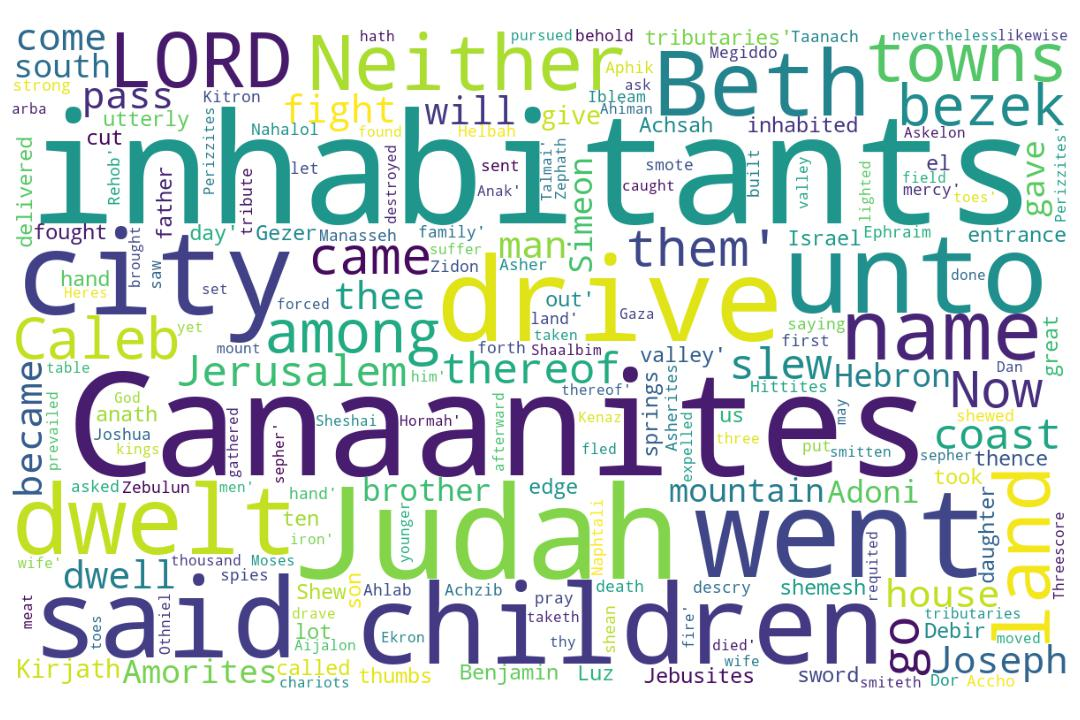
\includegraphics[width=\linewidth]{07OT-Judges/Judges1-WordCloud.jpg}
  \caption{Judges 1 Word Cloud}
  \label{fig:Judges 1 Word Cloud}
\end{figure}


\marginpar{\scriptsize \centering \fcolorbox{bone}{lime}{\textbf{THEYRE BACK}}\\ (Judges 1:1-36) \begin{compactenum}[I.][8]
    \item   A \textbf{Passing}  \index[scripture]{Judges!Jdg 01:01} (Jdg 1:1) 
    \item   The \textbf{Perrizites}  \index[scripture]{Judges!Jdg 01:04} \index[scripture]{Judges!Jdg 01:05} (Jdg 1:4, 5) 
    \item   The  \textbf{Pursuit}  \index[scripture]{Judges!Jdg 01:06} (Jdg 1:6) 
    \item   The  \textbf{Payback}  \index[scripture]{Judges!Jdg 01:07} (Jdg 1:7) 
    \item   The  \textbf{Pyrotechnics}  \index[scripture]{Judges!Jdg 01:08} (Jdg 1:8) 
    \item   The  \textbf{Prominent}  \index[scripture]{Judges!Jdg 01:10} (Jdg 1:10) 
    \item   The  \textbf{Promise}  \index[scripture]{Judges!Jdg 01:12} (Jdg 1:12) 
    \item   A Supposed \textbf{Problem}  \index[scripture]{Judges!Jdg 01:10} \index[scripture]{Judges!Jdg 01:20} (Jdg 1:10, 20) 
\end{compactenum}}

\marginpar{\scriptsize \centering \fcolorbox{bone}{yellow}{\textbf{UNFINISHED BUSINESS}}\\ (Judges 1:1-36) \begin{compactenum}[I.][8]
    \item  The \textbf{Canaanite Focus}  \index[scripture]{Judges!Jdg 01:01} (Jdg 1:1) 
    \item  \textbf{Compromised Faith}  \index[scripture]{Judges!Jdg 01:03}  (Jdg 1:3) 
    \item  \textbf{Casualities Forced}  \index[scripture]{Judges!Jdg 01:04} (Jdg 1:4) 
    \item  \textbf{Cut Feet}  \index[scripture]{Judges!Jdg 01:06-07} (Jdg 1:6-7) 
   \item  A \textbf{City on Fire}  \index[scripture]{Judges!Jdg 01:08} (Jdg 1:14-15) 
   \item  A \textbf{Call of a Female}  \index[scripture]{Judges!Jdg 01:14-15} (Jdg 1:14-15) 
    \item  \textbf{Caleb's Family}  \index[scripture]{Judges!Jdg 01:12} (Jdg 1:12) 
    \item  A \textbf{Call of a Female}  \index[scripture]{Judges!Jdg 01:14-15} (Jdg 1:14-15) 
\end{compactenum}}

\footnote{\textcolor[cmyk]{0.99998,1,0,0}{\hyperlink{TOC}{Return to end of Table of Contents.}}}\footnote{\href{https://audiobible.com/bible/judges_1.html}{\textcolor[cmyk]{0.99998,1,0,0}{Judges 1 Audio}}}\textcolor[cmyk]{0.99998,1,0,0}{Now after the \fcolorbox{bone}{lime}{death of Joshua} it came to pass, that the children of Israel asked the LORD, saying, Who shall go up for us against the Canaanites first, to fight against them?}
[2] \textcolor[cmyk]{0.99998,1,0,0}{And the LORD said, Judah shall go up: behold, I have delivered the land into his hand.}
[3] \textcolor[cmyk]{0.99998,1,0,0}{And Judah said unto Simeon his brother, Come up \fcolorbox{bone}{bone}{with} me into my lot, that we may fight against the Canaanites; and I likewise will go \fcolorbox{bone}{bone}{with} thee into thy lot. So Simeon went \fcolorbox{bone}{bone}{with} him.}
[4] \textcolor[cmyk]{0.99998,1,0,0}{And Judah went up; and the LORD delivered the Canaanites and the \fcolorbox{bone}{lime}{Perizzites} into their hand: and they slew of them in Bezek ten thousand men.}
[5] \textcolor[cmyk]{0.99998,1,0,0}{And they found Adoni-bezek in Bezek: and they fought against him, and they slew the Canaanites and the \fcolorbox{bone}{lime}{Perizzites}.}
[6] \textcolor[cmyk]{0.99998,1,0,0}{But Adoni-bezek fled; and they \fcolorbox{bone}{lime}{pursued} after him, and caught him, and cut off his thumbs and his great toes.}
[7] \textcolor[cmyk]{0.99998,1,0,0}{And Adoni-bezek said, Threescore and ten kings, having their thumbs and their great toes cut off, gathered \emph{their} \emph{meat} under my table: as I have done, so God hath \fcolorbox{bone}{lime}{requited} me. And they brought him to Jerusalem, and there he died.}
[8] \textcolor[cmyk]{0.99998,1,0,0}{Now the children of Judah had fought against Jerusalem, and had taken it, and smitten it \fcolorbox{bone}{bone}{with} the edge \fcolorbox{bone}{bone}{of the} sword, and set the city on \fcolorbox{bone}{lime}{fire}.}\\
\\
\P \textcolor[cmyk]{0.99998,1,0,0}{And afterward the children of Judah went down to fight against the Canaanites, that dwelt in the mountain, and in the south, and in the valley.}
[10] \textcolor[cmyk]{0.99998,1,0,0}{And Judah went against the Canaanites that dwelt in Hebron: (now the name of Hebron before \emph{was} Kirjath-arba:) and they slew \fcolorbox{bone}{lime}{Sheshai}, and \fcolorbox{bone}{lime}{Ahiman}, and \fcolorbox{bone}{lime}{Talmai}.}
[11] \textcolor[cmyk]{0.99998,1,0,0}{And from thence he went against the inhabitants of Debir: and the name of Debir before \emph{was} Kirjath-sepher:}
[12] \textcolor[cmyk]{0.99998,1,0,0}{And Caleb said, He that smiteth Kirjath-sepher, and taketh it, to him \fcolorbox{bone}{lime}{will I give} Achsah my daughter to wife.}
[13] \textcolor[cmyk]{0.99998,1,0,0}{And Othniel the son of Kenaz, Caleb's younger brother, took it: and he gave him Achsah his daughter to wife.}
[14] \textcolor[cmyk]{0.99998,1,0,0}{And it came to pass, when she came \emph{to} \emph{him}, that she moved him to ask of her father a field: and she lighted from off \emph{her} ass; and Caleb said unto her, What wilt thou?}
[15] \textcolor[cmyk]{0.99998,1,0,0}{And she said unto him, Give me a blessing: for thou hast given me a south land; give me also springs of water. And Caleb gave her the upper springs and the nether springs.}\\
\\
\P \textcolor[cmyk]{0.99998,1,0,0}{And the children \fcolorbox{bone}{bone}{of the} Kenite, Moses' father in law, went up out \fcolorbox{bone}{bone}{of the} city of palm trees \fcolorbox{bone}{bone}{with} the children of Judah into the wilderness of Judah, which \emph{lieth} in the south of Arad; and they went and dwelt among the people.}
[17] \textcolor[cmyk]{0.99998,1,0,0}{And Judah went \fcolorbox{bone}{bone}{with} Simeon his brother, and they slew the Canaanites that inhabited Zephath, and utterly destroyed it. And the name \fcolorbox{bone}{bone}{of the} city was called Hormah.}
[18] \textcolor[cmyk]{0.99998,1,0,0}{Also Judah took Gaza \fcolorbox{bone}{bone}{with} the coast thereof, and Askelon \fcolorbox{bone}{bone}{with} the coast thereof, and Ekron \fcolorbox{bone}{bone}{with} the coast thereof.}
[19] \textcolor[cmyk]{0.99998,1,0,0}{And the LORD was \fcolorbox{bone}{bone}{with} Judah; and he drave out \emph{the} \emph{inhabitants} \emph{of} the mountain; but could not drive out the inhabitants \fcolorbox{bone}{bone}{of the} valley, because they had chariots of iron.}
[20] \textcolor[cmyk]{0.99998,1,0,0}{And they gave Hebron unto Caleb, as Moses said: and he expelled thence the three sons of Anak.}
[21] \textcolor[cmyk]{0.99998,1,0,0}{And the children of Benjamin did not drive out the Jebusites that inhabited Jerusalem; but the Jebusites dwell \fcolorbox{bone}{bone}{with} the children of Benjamin in Jerusalem unto this day.}\\
\\
\P \textcolor[cmyk]{0.99998,1,0,0}{And the house of Joseph, they also went up against Beth-el: and the LORD \emph{was} \fcolorbox{bone}{bone}{with} them.}
[23] \textcolor[cmyk]{0.99998,1,0,0}{And the house of Joseph sent to descry Beth-el. (Now the name \fcolorbox{bone}{bone}{of the} city before \emph{was} Luz.)}
[24] \textcolor[cmyk]{0.99998,1,0,0}{And the spies saw a man come forth out \fcolorbox{bone}{bone}{of the} city, and they said unto him, Shew us, we pray thee, the entrance into the city, and we will shew thee mercy.}
[25] \textcolor[cmyk]{0.99998,1,0,0}{And when he shewed them the entrance into the city, they smote the city \fcolorbox{bone}{bone}{with} the edge \fcolorbox{bone}{bone}{of the} sword; but they let go the man and all his family.}
[26] \textcolor[cmyk]{0.99998,1,0,0}{And the man went into the land \fcolorbox{bone}{bone}{of the} Hittites, and built a city, and called the name thereof Luz: which \emph{is} the name thereof unto this day.}\\
\\
\P \textcolor[cmyk]{0.99998,1,0,0}{Neither did Manasseh drive out \emph{the} \emph{inhabitants} \emph{of} Beth-shean and her towns, nor Taanach and her towns, nor the inhabitants of Dor and her towns, nor the inhabitants of Ibleam and her towns, nor the inhabitants of Megiddo and her towns: but the Canaanites would dwell in that land.}
[28] \textcolor[cmyk]{0.99998,1,0,0}{And it came to pass, when Israel was strong, that they put the Canaanites to tribute, and did not utterly drive them out.}\\
\\
\P \textcolor[cmyk]{0.99998,1,0,0}{Neither did Ephraim drive out the Canaanites that dwelt in Gezer; but the Canaanites dwelt in Gezer among them.}\\
\\
\P \textcolor[cmyk]{0.99998,1,0,0}{Neither did Zebulun drive out the inhabitants of Kitron, nor the inhabitants of Nahalol; but the Canaanites dwelt among them, and became tributaries.}
[31] \textcolor[cmyk]{0.99998,1,0,0}{Neither did Asher drive out the inhabitants of Accho, nor the inhabitants of Zidon, nor of Ahlab, nor of Achzib, nor of Helbah, nor of Aphik, nor of Rehob:}
[32] \textcolor[cmyk]{0.99998,1,0,0}{But the Asherites dwelt among the Canaanites, the inhabitants \fcolorbox{bone}{bone}{of the} land: for they did not drive them out.}\\
\\
\P \textcolor[cmyk]{0.99998,1,0,0}{Neither did Naphtali drive out the inhabitants of Beth-shemesh, nor the inhabitants of Beth-anath; but he dwelt among the Canaanites, the inhabitants \fcolorbox{bone}{bone}{of the} land: nevertheless the inhabitants of Beth-shemesh and of Beth-anath became tributaries unto them.}
[34] \textcolor[cmyk]{0.99998,1,0,0}{And the Amorites forced the children of Dan into the mountain: for they would not suffer them to come down to the valley:}
[35] \textcolor[cmyk]{0.99998,1,0,0}{But the Amorites would dwell in mount Heres in Aijalon, and in Shaalbim: yet the hand \fcolorbox{bone}{bone}{of the} house of Joseph prevailed, so that they became tributaries.}
[36] \textcolor[cmyk]{0.99998,1,0,0}{And the coast \fcolorbox{bone}{bone}{of the} Amorites \emph{was} from the going up to Akrabbim, from the rock, and upward.}
\chapter{Judges 2}

\begin{figure}
  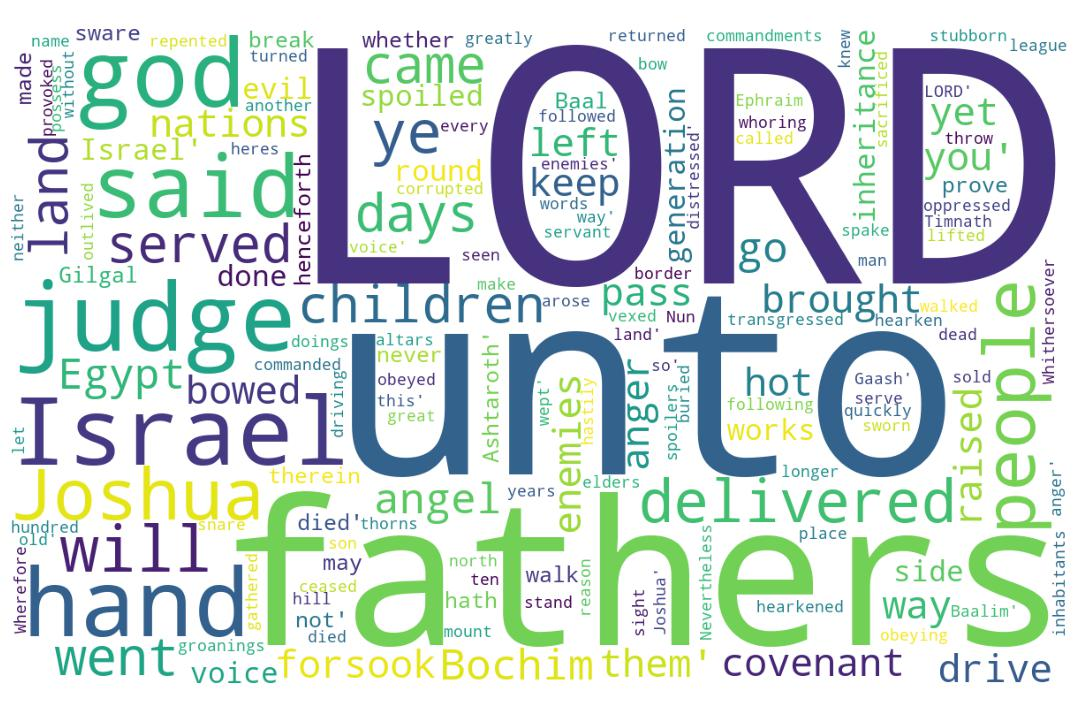
\includegraphics[width=\linewidth]{07OT-Judges/Judges2-WordCloud.jpg}
  \caption{Judges 2 Word Cloud}
  \label{fig:Judges 2 Word Cloud}
\end{figure}


\marginpar{\scriptsize \centering \fcolorbox{bone}{lime}{\textbf{COLLAPSE}}\\ (Judges 2:1-23) \begin{compactenum}[I.][8]
    \item   The \textbf{Covenant}  \index[scripture]{Judges!Jdg 02:01} (Jdg 2:1) 
    \item   The \textbf{Compromise}  \index[scripture]{Judges!Jdg 02:02} (Jdg 2:2) 
    \item   The \textbf{Crocodile Tears}  \index[scripture]{Judges!Jdg 02:04} (Jdg 2:4) 
    \item   The \textbf{Decline}  \index[scripture]{Judges!Jdg 02:10} (Jdg 2:10) 
    \item    \textbf{Corruption}  \index[scripture]{Judges!Jdg 02:11} (Jdg 2:11) 
    \item    \textbf{Collapse}  \index[scripture]{Judges!Jdg 02:12} (Jdg 2:12) 
    \item   The \textbf{Acrimony}  \index[scripture]{Judges!Jdg 02:14}\index[scripture]{Judges!Jdg 02:20} (Jdg 2:14, 20) 
    \item    \textbf{Champions}  \index[scripture]{Judges!Jdg 02:16} (Jdg 2:16) 
\end{compactenum}}

\marginpar{\scriptsize \centering \fcolorbox{bone}{yellow}{\textbf{HAVE IT YOUR WAY}}\\ (Judges 2:12-23) \begin{compactenum}[I.][8]
    \item   \textbf{Forsaking}  \index[scripture]{Judges!Jdg 02:12} (Jdg 2:12) 
    \item   \textbf{Following} other Gods  \index[scripture]{Judges!Jdg 02:12} (Jdg 2:12) 
    \item   \textbf{Falling Down}  \index[scripture]{Judges!Jdg 02:12} (Jdg 2:12) 
    \item   The \textbf{False}  Ones \index[scripture]{Judges!Jdg 02:13} (Jdg 2:13) 
    \item   \textbf{Enflaming} Anger \index[scripture]{Judges!Jdg 02:14} 
              \index[scripture]{Judges!Jdg 02:20} (Jdg 2:14, 20) 
    \item   The \textbf{Fruit}  Ones \index[scripture]{Judges!Jdg 02:16} (Jdg 2:16) 
    \item   \textbf{Five} Lords\index[scripture]{Judges!Jdg 03:03} (Jdg 3:3) 
\end{compactenum}}

\footnote{\textcolor[cmyk]{0.99998,1,0,0}{\hyperlink{TOC}{Return to end of Table of Contents.}}}\footnote{\href{https://audiobible.com/bible/judges_2.html}{\textcolor[cmyk]{0.99998,1,0,0}{Judges 2 Audio}}}\textcolor[cmyk]{0.99998,1,0,0}{And an angel of the LORD came up from Gilgal to Bochim, and said, I made you to go up out of Egypt, and have brought you \fcolorbox{bone}{bone}{unto} the land which I sware \fcolorbox{bone}{bone}{unto} your fathers; and I said, I will never break my \fcolorbox{bone}{lime}{covenant} with you.}
[2] \textcolor[cmyk]{0.99998,1,0,0}{And ye shall make no \fcolorbox{bone}{lime}{league} with the inhabitants of this land; ye shall throw down their altars: but ye have not obeyed my voice: why have ye done this?}
[3] \textcolor[cmyk]{0.99998,1,0,0}{Wherefore I also said, I will not drive them out from before you; but they shall be \emph{as} \emph{thorns} in your sides, and their gods shall be a snare \fcolorbox{bone}{bone}{unto} you.}
[4] \textcolor[cmyk]{0.99998,1,0,0}{And it came to pass, when the angel of the LORD spake these words \fcolorbox{bone}{bone}{unto} all the children of Israel, that the people lifted up their voice, and \fcolorbox{bone}{lime}{wept}.}
[5] \textcolor[cmyk]{0.99998,1,0,0}{And they called the name of that place Bochim: and they sacrificed there \fcolorbox{bone}{bone}{unto} the LORD.}\\
\\
\P \textcolor[cmyk]{0.99998,1,0,0}{And when Joshua had let the people go, the children of Israel went every man \fcolorbox{bone}{bone}{unto} his inheritance to possess the land.}
[7] \textcolor[cmyk]{0.99998,1,0,0}{And the people served the LORD all the days of Joshua, and all the days of the elders that outlived Joshua, who had seen all the great works of the LORD, that he did for Israel.}
[8] \textcolor[cmyk]{0.99998,1,0,0}{And Joshua the son of Nun, the servant of the LORD, died, \emph{being} an hundred and ten years old.}
[9] \textcolor[cmyk]{0.99998,1,0,0}{And they buried him in the border of his inheritance in Timnath-heres, in the mount of Ephraim, on the north side of the hill Gaash.}
[10] \textcolor[cmyk]{0.99998,1,0,0}{And also all that generation were gathered \fcolorbox{bone}{bone}{unto} their fathers: and there arose another generation after them, which \fcolorbox{bone}{lime}{knew not} the LORD, nor yet the works which he had done for Israel.}\\
\\
\P \textcolor[cmyk]{0.99998,1,0,0}{And the children of Israel did evil in the sight of the LORD, and \fcolorbox{bone}{lime}{served} \fcolorbox{bone}{lime}{Baalim}:}
[12] \textcolor[cmyk]{0.99998,1,0,0}{And they forsook the LORD God of their fathers, which brought them out of the land of Egypt, and followed other gods, of the gods of the people that \emph{were} round about them, and \fcolorbox{bone}{lime}{bowed themselves} \fcolorbox{bone}{bone}{unto} them, and provoked the LORD to anger.}
[13] \textcolor[cmyk]{0.99998,1,0,0}{And they forsook the LORD, and served Baal and Ashtaroth.}\\
\\
\P \textcolor[cmyk]{0.99998,1,0,0}{And the anger of the LORD was hot against Israel, and he \fcolorbox{bone}{lime}{delivered them} into the hands of spoilers that spoiled them, and he sold them into the hands of their enemies round about, so that they could not any longer stand before their enemies.}
[15] \textcolor[cmyk]{0.99998,1,0,0}{Whithersoever they went out, the hand of the LORD was against them for evil, as the LORD had said, and as the LORD had sworn \fcolorbox{bone}{bone}{unto} them: and they were greatly distressed.}\\
\\
\P \textcolor[cmyk]{0.99998,1,0,0}{Nevertheless the LORD raised up \fcolorbox{bone}{lime}{judges}, which delivered them out of the hand of those that spoiled them.}
[17] \textcolor[cmyk]{0.99998,1,0,0}{And yet they would not hearken \fcolorbox{bone}{bone}{unto} their judges, but they went a whoring after other gods, and bowed themselves \fcolorbox{bone}{bone}{unto} them: they turned quickly out of the way which their fathers walked in, obeying the commandments of the LORD; \emph{but} they did not so.}
[18] \textcolor[cmyk]{0.99998,1,0,0}{And when the LORD raised them up judges, then the LORD was with the judge, and delivered them out of the hand of their enemies all the days of the judge: for it repented the LORD because of their groanings by reason of them that oppressed them and vexed them.}
[19] \textcolor[cmyk]{0.99998,1,0,0}{And it came to pass, when the judge was dead, \emph{that} they returned, and corrupted \emph{themselves} more than their fathers, in following other gods to serve them, and to bow down \fcolorbox{bone}{bone}{unto} them; they ceased not from their own doings, nor from their stubborn way.}\\
\\
\P \textcolor[cmyk]{0.99998,1,0,0}{And the anger of the LORD was hot against Israel; and he said, Because that this people hath transgressed my covenant which I commanded their fathers, and have not hearkened \fcolorbox{bone}{bone}{unto} my voice;}
[21] \textcolor[cmyk]{0.99998,1,0,0}{I also will not henceforth drive out any from before them of the nations which Joshua left when he died:}
[22] \textcolor[cmyk]{0.99998,1,0,0}{That through them I may prove Israel, whether they will keep the way of the LORD to walk therein, as their fathers did keep \emph{it}, or not.}
[23] \textcolor[cmyk]{0.99998,1,0,0}{Therefore the LORD left those nations, without driving them out hastily; neither delivered he them into the hand of Joshua.}
\chapter{Judges 3}

\begin{figure}
  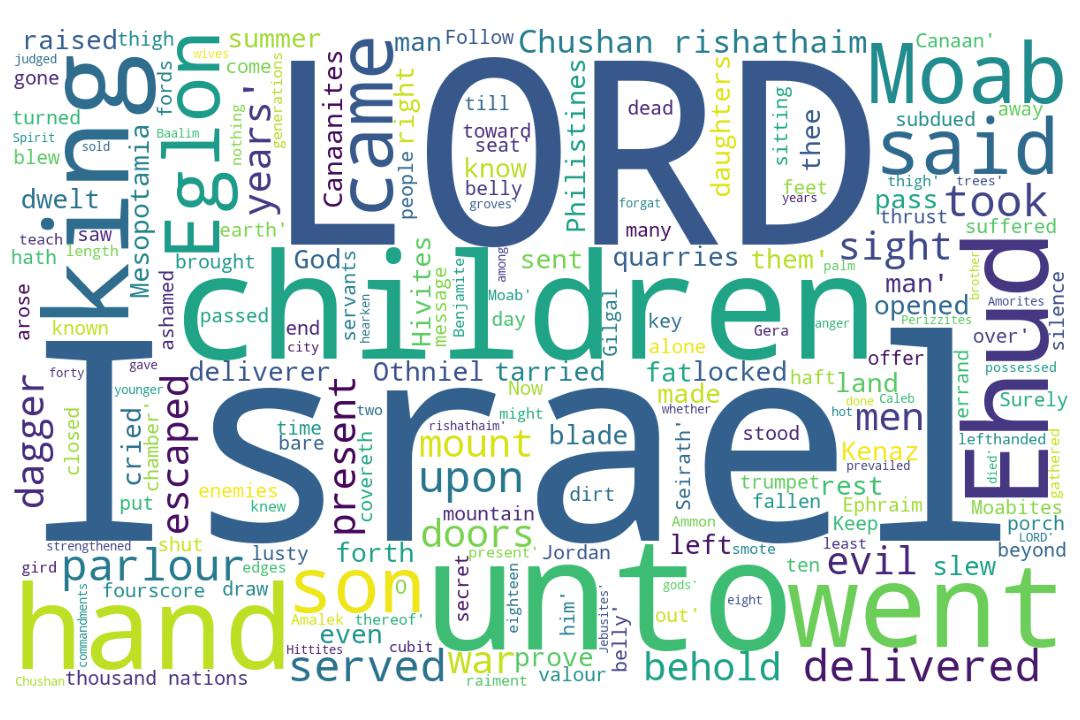
\includegraphics[width=\linewidth]{07OT-Judges/Judges3-WordCloud.jpg}
  \caption{Judges 3 Word Cloud}
  \label{fig:Judges 3 Word Cloud}
\end{figure}

\marginpar{\scriptsize \centering \fcolorbox{bone}{lime}{\textbf{A CYCLE APPEARS}}\\ (Judges 3:1-7) \begin{compactenum}[I.][8]
    \item   The \textbf{Thorns}  \index[scripture]{Judges!Jdg 03:01} (Jdg 3:1) 
    \item   The \textbf{Teaching}  \index[scripture]{Judges!Jdg 03:02} (Jdg 3:2) 
    \item    \textbf{Testing}  \index[scripture]{Judges!Jdg 03:04} (Jdg 3:4) 
    \item   A \textbf{Toxin}  \index[scripture]{Judges!Jdg 03:06} (Jdg 3:6) 
    \item   The \textbf{Transgressions}  \index[scripture]{Judges!Jdg 03:07} (Jdg 3:7) 
    \item   Ruined \textbf{Theology}  \index[scripture]{Judges!Jdg 03:07} (Jdg 3:7) 
    \item   The \textbf{Theme}  the cycle of sin, judgmentm repentance, rescue % \index[scripture]{Judges!Jdg 03:01} (Judges 3:1) 
\end{compactenum}}


\marginpar{\scriptsize \centering \fcolorbox{bone}{yellow}{\textbf{ROUND 1}}\\ (Judges 3:5-11) 
\begin{compactenum}[I.][8]
    \item   \textbf{Six} Enemies \index[scripture]{Judges!Jdg 03:05} (Jdg 3:5) 
    \item   \textbf{Sons \& Daughters}  \index[scripture]{Judges!Jdg 03:06} (Jdg 3:6)  
    \item   \textbf{Service} to Balaam \index[scripture]{Judges!Jdg 03:07} (Jdg 3:7)  
    \item   \textbf{Sold} to Mesopotamia \index[scripture]{Judges!Jdg 03:08} (Jdg 3:8)  
    \item   Israel's  \textbf{Supplication} \index[scripture]{Judges!Jdg 03:09} (Jdg 3:9)  
    \item   Othniel, the \textbf{Savior} \index[scripture]{Judges!Jdg 03:09} (Jdg 3:9)  
    \item   \textbf{Stillness} for 40 Years \index[scripture]{Judges!Jdg 03:11} (Jdg 3:11)  
\end{compactenum}}




\footnote{\textcolor[cmyk]{0.99998,1,0,0}{\hyperlink{TOC}{Return to end of Table of Contents.}}}\footnote{\href{https://audiobible.com/bible/judges_3.html}{\textcolor[cmyk]{0.99998,1,0,0}{Judges 3 Audio}}}\textcolor[cmyk]{0.99998,1,0,0}{Now these \emph{are} the nations which the LORD left, \fcolorbox{bone}{lime}{to prove} Israel by them, \emph{even} as many \emph{of} \emph{Israel} as had not known all the wars of Canaan;}
[2] \textcolor[cmyk]{0.99998,1,0,0}{Only that the generations of the children of Israel might \fcolorbox{bone}{lime}{know}, to teach them war, at the least such as before knew nothing thereof;}
[3] \textcolor[cmyk]{0.99998,1,0,0}{\emph{Namely}, five lords of the Philistines, and all the Canaanites, and the Sidonians, and the Hivites that dwelt in mount Lebanon, from mount Baal-hermon unto the entering in of Hamath.}
[4] \textcolor[cmyk]{0.99998,1,0,0}{And they were to \fcolorbox{bone}{lime}{prove} Israel by them, to know whether they would hearken unto the commandments of the LORD, which he commanded their fathers by the hand of Moses.}\\
\\
\P \textcolor[cmyk]{0.99998,1,0,0}{And the children of Israel dwelt among the \fcolorbox{bone}{yellow}{Canaanites}, \fcolorbox{bone}{yellow}{Hittites}, and \fcolorbox{bone}{yellow}{Amorites}, and \fcolorbox{bone}{yellow}{Perizzites}, and \fcolorbox{bone}{yellow}{Hivites}, and \fcolorbox{bone}{yellow}{Jebusites}:}
[6] \textcolor[cmyk]{0.99998,1,0,0}{And they took their \fcolorbox{bone}{lime}{daughters} to be their wives, and gave their daughters to their \fcolorbox{bone}{lime}{sons}, and served their gods.}
[7] \textcolor[cmyk]{0.99998,1,0,0}{And the children of Israel did \fcolorbox{bone}{lime}{evil} in the sight of the LORD, and \fcolorbox{bone}{lime}{forgat} the LORD their God, and \fcolorbox{bone}{lime}{served} Baalim and the groves.}\\
\\
\P \textcolor[cmyk]{0.99998,1,0,0}{Therefore the anger of the LORD was hot against Israel, and he sold them into the hand of Chushan-rishathaim king of Mesopotamia: and the children of Israel served Chushan-rishathaim eight years.}
[9] \textcolor[cmyk]{0.99998,1,0,0}{And when the children of Israel \fcolorbox{bone}{yellow}{cried} unto the LORD, the LORD raised up a deliverer to the children of Israel, who delivered them, \emph{even} \fcolorbox{bone}{yellow}{Othniel} the son of Kenaz, Caleb's younger brother.}
[10] \textcolor[cmyk]{0.99998,1,0,0}{And the Spirit of the LORD came upon him, and he judged Israel, and went out to war: and the LORD delivered Chushan-rishathaim king of Mesopotamia into his hand; and his hand prevailed against Chushan-rishathaim.}
[11] \textcolor[cmyk]{0.99998,1,0,0}{And the land had \fcolorbox{bone}{yellow}{rest} forty years. And Othniel the son of Kenaz died.}\\
\\
\P \textcolor[cmyk]{0.99998,1,0,0}{And the children of Israel did evil again in the sight of the LORD: and the LORD strengthened Eglon the king of Moab against Israel, because they had done evil in the sight of the LORD.}
[13] \textcolor[cmyk]{0.99998,1,0,0}{And he gathered unto him the children of Ammon and Amalek, and went and smote Israel, and possessed the city of palm trees.}
[14] \textcolor[cmyk]{0.99998,1,0,0}{So the children of Israel served Eglon the king of Moab eighteen years.}
[15] \textcolor[cmyk]{0.99998,1,0,0}{But when the children of Israel cried unto the LORD, the LORD raised them up a deliverer, Ehud the son of Gera, a Benjamite, a man lefthanded: and by him the children of Israel sent a present unto Eglon the king of Moab.}
[16] \textcolor[cmyk]{0.99998,1,0,0}{But Ehud made him a dagger which had two edges, of a cubit length; and he did gird it under his raiment upon his right thigh.}
[17] \textcolor[cmyk]{0.99998,1,0,0}{And he brought the present unto Eglon king of Moab: and Eglon \emph{was} a very fat man.}
[18] \textcolor[cmyk]{0.99998,1,0,0}{And when he had made an end to offer the present, he sent away the people that bare the present.}
[19] \textcolor[cmyk]{0.99998,1,0,0}{But he himself turned again from the quarries that \emph{were} by Gilgal, and said, I have a secret errand unto thee, O king: who said, Keep silence. And all that stood by him went out from him.}
[20] \textcolor[cmyk]{0.99998,1,0,0}{And Ehud came unto him; and he was sitting in a summer parlour, which he had for himself alone. And Ehud said, I have a message from God unto thee. And he arose out of \emph{his} seat.}
[21] \textcolor[cmyk]{0.99998,1,0,0}{And Ehud put forth his left hand, and took the dagger from his right thigh, and thrust it into his belly:}
[22] \textcolor[cmyk]{0.99998,1,0,0}{And the haft also went in after the blade; and the fat closed upon the blade, so that he could not draw the dagger out of his belly; and the dirt came out.}
[23] \textcolor[cmyk]{0.99998,1,0,0}{Then Ehud went forth through the porch, and shut the doors of the parlour upon him, and locked them.}
[24] \textcolor[cmyk]{0.99998,1,0,0}{When he was gone out, his servants came; and when they saw that, behold, the doors of the parlour \emph{were} locked, they said, Surely he covereth his feet in his summer chamber.}
[25] \textcolor[cmyk]{0.99998,1,0,0}{And they tarried till they were ashamed: and, behold, he opened not the doors of the parlour; therefore they took a key, and opened \emph{them}: and, behold, their lord \emph{was} fallen down dead on the earth.}
[26] \textcolor[cmyk]{0.99998,1,0,0}{And Ehud escaped while they tarried, and passed beyond the quarries, and escaped unto Seirath.}
[27] \textcolor[cmyk]{0.99998,1,0,0}{And it came to pass, when he was come, that he blew a trumpet in the mountain of Ephraim, and the children of Israel went down with him from the mount, and he before them.}
[28] \textcolor[cmyk]{0.99998,1,0,0}{And he said unto them, Follow after me: for the LORD hath delivered your enemies the Moabites into your hand. And they went down after him, and took the fords of Jordan toward Moab, and suffered not a man to pass over.}
[29] \textcolor[cmyk]{0.99998,1,0,0}{And they slew of Moab at that time about ten thousand men, all lusty, and all men of valour; and there escaped not a man.}
[30] \textcolor[cmyk]{0.99998,1,0,0}{So Moab was subdued that day under the hand of Israel. And the land had rest fourscore years.}\\
\\
\P \textcolor[cmyk]{0.99998,1,0,0}{And after him was Shamgar the son of Anath, which slew of the Philistines six hundred men with an ox goad: and he also delivered Israel.}

\chapter{Psalm 73}

\begin{figure}
  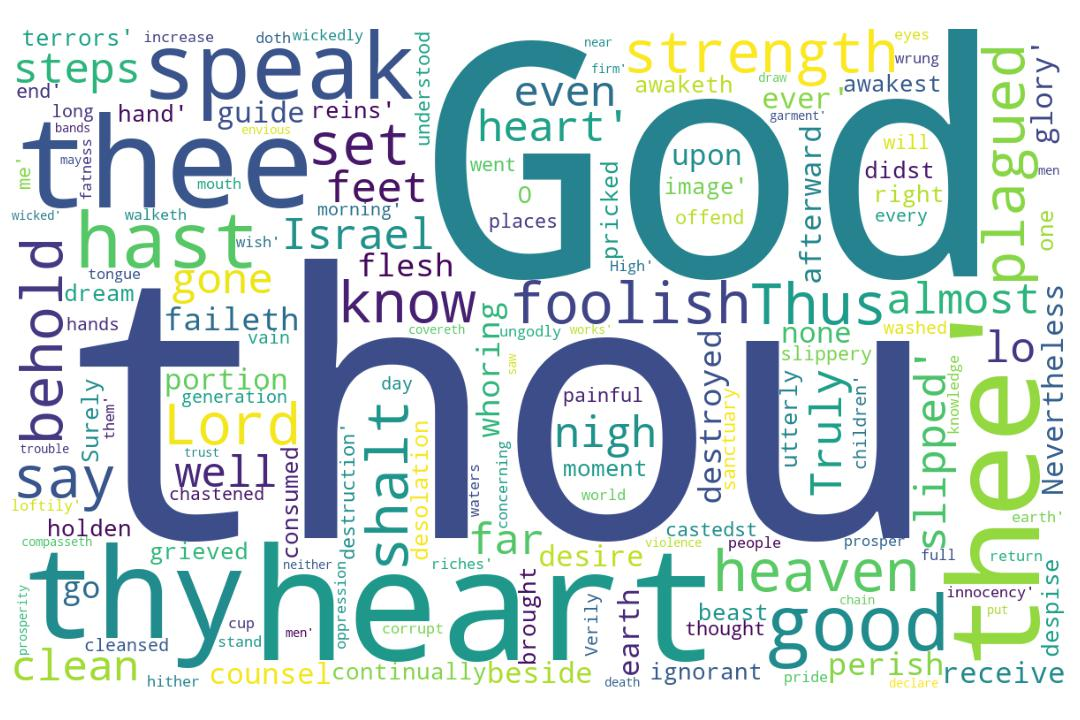
\includegraphics[width=\linewidth]{19OT-Psalms/Psalm73-WordCloud.jpg}
  \caption{Psalm 73 Word Cloud}
  \label{fig:Psalm 73 word Cloud}
\end{figure}

\marginpar{\scriptsize \centering \fcolorbox{bone}{lime}{\textbf{A GOOD GOD}}\\ (Psalm 73:1-28) \begin{compactenum}[I.][8]
    \item \textbf{A Clean Heart} \index[scripture]{Psalms!Psa 073:01}(Psa 73:1)
    \item \textbf{Compassing Hubris} \index[scripture]{Psalms!Psa 073:06}(pride) (Psa 73:6)
    \item \textbf{Corrupt Humanity} \index[scripture]{Psalms!Psa 073:08}(Psa 73:8)
    \item \textbf{Cleansed Hearts} \index[scripture]{Psalms!Psa 073:13}(Psa 73:13)
    \item \textbf{A Cast-Down Heap} \index[scripture]{Psalms!Psa 073:18}(Psa 73:18)
    \item \textbf{A Consuming Horror} \index[scripture]{Psalms!Psa 073:19}(Psa 73:19)
    \item \textbf{A Continual Help} \index[scripture]{Psalms!Psa 073:23}(Psa 73:23)
\end{compactenum}}
    
\marginpar{
\scriptsize \centering 
\fcolorbox{bone}{yellow}{\textbf{THE WICKED \& THEIR PROSPERITY}}\\ (Psalm 73:1-28) \begin{compactenum}[I.][8]
    \item Their \textbf{Compassing} \index[scripture]{Psalms!Psa 073:06}(Psa 73:6)
    \item Their \textbf{Comfort} \index[scripture]{Psalms!Psa 073:07}(Psa 73:7)
    \item Their \textbf{Corruption} \index[scripture]{Psalms!Psa 073:08}(Psa 73:8)
    \item Their \textbf{Concern} \index[scripture]{Psalms!Psa 073:06}(Psa 73:6)
    \item Their \textbf{Conceit} \index[scripture]{Psalms!Psa 073:11}(Psa 73:11)
    \item Their \textbf{Cup} \index[scripture]{Psalms!Psa 073:10}(Psa 73:10)
    \item Their \textbf{Consumption} \index[scripture]{Psalms!Psa 073:18}(Psa 73:18)
\end{compactenum}}

\marginpar{
\scriptsize \centering 
\fcolorbox{bone}{blue}{\textbf{\textcolor[cmyk]{0,0,0,0}{TWO KINDS OF PEOPLE}}}\\
(Psalm 73:1-28) 
\begin{compactenum}[I.][8]
    \item (The Wicked Have) \textbf{Compassing Pride} \index[scripture]{Psalms!Psa 073:06}(Psa 73:6)
    \item (The Wicked Have) \textbf{Covering Violence} \index[scripture]{Psalms!Psa 073:06}(Psa 73:6)
    \item (The Wicked Have) \textbf{Corrupt Speech} \index[scripture]{Psalms!Psa 073:08}(Psa 73:8)
    \item (The Wicked Have) \textbf{A Clear End} \index[scripture]{Psalms!Psa 073:10}(Psa 73:10)
    \item (The Wicked Will Be) \textbf{Cast Down} \index[scripture]{Psalms!Psa 073:18}(Psa 73:18)
    \item (The Wicked Will Be) \textbf{Consumed with Terrors} \index[scripture]{Psalms!Psa 073:19}(Psa 73:19)
    \item (God's People Have) \textbf{Clean Hearts} \index[scripture]{Psalms!Psa 073:01}(Psa 73:1)
    \item (God's People Have God's) \textbf{Continual Presence} \index[scripture]{Psalms!Psa 073:23}(Psa 73:23)
\end{compactenum} }



\footnote{\textcolor[cmyk]{0.99998,1,0,0}{\hyperlink{TOC}{Return to end of Table of Contents.}}}\footnote{\href{https://audiobible.com/bible/psalms_73.html}{\textcolor[cmyk]{0.99998,1,0,0}{Psalm 73 Audio}}}\textcolor[cmyk]{0.99998,1,0,0}{A Psalm of Asaph}\\
\\
\textcolor[cmyk]{0.99998,1,0,0}{Truly God \emph{is} good to Israel, \emph{even} to such as are of a \fcolorbox{bone}{lime}{clean heart}.}
[2] \textcolor[cmyk]{0.99998,1,0,0}{But as for me, my feet were almost gone; my steps had well nigh slipped.}
[3] \textcolor[cmyk]{0.99998,1,0,0}{For I was envious at \fcolorbox{bone}{bone}{the} foolish, \emph{when} I saw \fcolorbox{bone}{bone}{the} prosperity of \fcolorbox{bone}{bone}{the} wicked.}
[4] \textcolor[cmyk]{0.99998,1,0,0}{For \emph{there} \emph{are} no bands in their death: but their strength \emph{is} firm.}
[5] \textcolor[cmyk]{0.99998,1,0,0}{They \emph{are} not in trouble \emph{as} \emph{other} men; neither are they plagued like \emph{other} men.}
[6] \textcolor[cmyk]{0.99998,1,0,0}{Therefore pride \fcolorbox{bone}{lime}{compasseth} them about as a chain; violence covereth them \emph{as} a garment.}
[7] \textcolor[cmyk]{0.99998,1,0,0}{Their eyes stand out with fatness: they have more than heart could wish.}
[8] \textcolor[cmyk]{0.99998,1,0,0}{They are \fcolorbox{bone}{lime}{corrupt}, and speak wickedly \emph{concerning} oppression: they speak loftily.}
[9] \textcolor[cmyk]{0.99998,1,0,0}{They set their mouth against \fcolorbox{bone}{bone}{the} heavens, and their tongue walketh through \fcolorbox{bone}{bone}{the} earth.}
[10] \textcolor[cmyk]{0.99998,1,0,0}{Therefore his people return hither: and waters of a full \emph{cup} are wrung out to them.}
[11] \textcolor[cmyk]{0.99998,1,0,0}{And they say, How doth God know? and is there knowledge in \fcolorbox{bone}{bone}{the} most High?}
[12] \textcolor[cmyk]{0.99998,1,0,0}{Behold, these \emph{are} \fcolorbox{bone}{bone}{the} ungodly, who prosper in \fcolorbox{bone}{bone}{the} world; they increase \emph{in} riches.}
[13] \textcolor[cmyk]{0.99998,1,0,0}{Verily I have \fcolorbox{bone}{lime}{cleansed} my heart \emph{in} vain, and washed my hands in innocency.}
[14] \textcolor[cmyk]{0.99998,1,0,0}{For all \fcolorbox{bone}{bone}{the} day long have I been plagued, and chastened every morning.}
[15] \textcolor[cmyk]{0.99998,1,0,0}{If I say, I will speak thus; behold, I should offend \emph{against} \fcolorbox{bone}{bone}{the} generation of thy children.}
[16] \textcolor[cmyk]{0.99998,1,0,0}{When I thought to know this, it \emph{was} too painful for me;}
[17] \textcolor[cmyk]{0.99998,1,0,0}{Until I went into \fcolorbox{bone}{bone}{the} sanctuary of God; \emph{then} understood I their end.}
[18] \textcolor[cmyk]{0.99998,1,0,0}{Surely thou didst set them in slippery places: thou \fcolorbox{bone}{lime}{castedst} them down into destruction.}
[19] \textcolor[cmyk]{0.99998,1,0,0}{How are they \emph{brought} into desolation, as in a moment! they are utterly \fcolorbox{bone}{lime}{consumed} with terrors.}
[20] \textcolor[cmyk]{0.99998,1,0,0}{As a dream when \emph{one} awaketh; \emph{so}, O Lord, when thou awakest, thou shalt despise their image.}
[21] \textcolor[cmyk]{0.99998,1,0,0}{Thus my heart was grieved, and I was pricked in my reins.}
[22] \textcolor[cmyk]{0.99998,1,0,0}{So foolish \emph{was} I, and ignorant: I was \emph{as} a beast before thee.}
[23] \textcolor[cmyk]{0.99998,1,0,0}{Nevertheless I \emph{am} \fcolorbox{bone}{lime}{continually} with thee: thou hast holden \emph{me} by my right hand.}
[24] \textcolor[cmyk]{0.99998,1,0,0}{Thou shalt guide me with thy counsel, and afterward receive me \emph{to} glory.}
[25] \textcolor[cmyk]{0.99998,1,0,0}{Whom have I in heaven \emph{but} \emph{thee}? and \emph{there} \emph{is} none upon earth \emph{that} I desire beside thee.}
[26] \textcolor[cmyk]{0.99998,1,0,0}{My flesh and my heart faileth: \emph{but} God \emph{is} \fcolorbox{bone}{bone}{the} strength of my heart, and my portion for ever.}
[27] \textcolor[cmyk]{0.99998,1,0,0}{For, lo, they that are far from thee shall perish: thou hast destroyed all them that go a whoring from thee.}
[28] \textcolor[cmyk]{0.99998,1,0,0}{But \emph{it} \emph{is} good for me to draw near to God: I have put my trust in \fcolorbox{bone}{bone}{the} Lord GOD, that I may declare all thy works.}

\chapter{Proverb 14}

\begin{figure}
  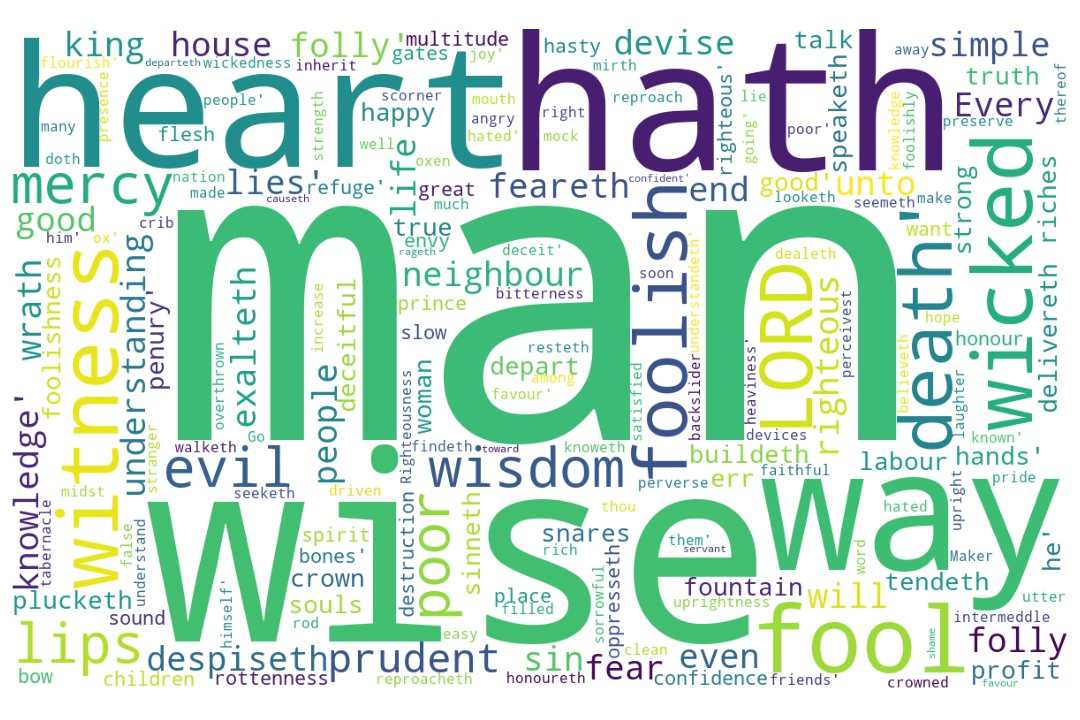
\includegraphics[width=\linewidth]{20OT-Proverbs/Proverb14-WordCloud.jpg}
  \caption{Proverb 14 Word Cloud}
  \label{fig:Proverb 14 Word Cloud}
\end{figure}

\marginpar{\scriptsize \centering \fcolorbox{bone}{lime}{\textbf{WHAT A FOOL DOES}}\\ (Proverbs 14:1-35) \begin{compactenum}[I.][8]
    \item \textbf{Derides Righteousness} (Proverbs 14:9 --  verse with 13 words) \index[scripture]{Proverbs!Pro 14:09}(Pro 14:9)
    \item \textbf{Dealeth in Anger} \index[scripture]{Proverbs!Pro 14:17}(Pro 14:17)
    \item \textbf{Despises Good} \index[scripture]{Proverbs!Pro 14:01, 21}(Pro 14:1, 21)
    \item \textbf{Devises Evil} \index[scripture]{Proverbs!Pro 14:22}(Pro 14:22)
    \item \textbf{Deceives Souls} \index[scripture]{Proverbs!Pro 14:25}(Pro 14:25)
    \item \textbf{Destroys Order} \index[scripture]{Proverbs!Pro 14:28}(Pro 14:28)
    \item \textbf{Deserves Destruction} \index[scripture]{Proverbs!Pro 14:35}(Pro 14:35)
\end{compactenum}}

\marginpar{\scriptsize \centering \fcolorbox{bone}{yellow}{\textbf{7 KINDS OF MEN}}\\ (Proverbs 14:1-35) \begin{compactenum}[I.][8]
    \item The \textbf{False} Man \index[scripture]{Proverbs!Pro 14:05}(Pro 14:5)
    \item The \textbf{Faithful} Man \index[scripture]{Proverbs!Pro 14:05}(Pro 14:5)
    \item The \textbf{Foolish} Man \index[scripture]{Proverbs!Pro 14:08} \index[scripture]{Proverbs!Pro 14:09}  \index[scripture]{Proverbs!Pro 14:24} \index[scripture]{Proverbs!Pro 14:33} (Pro 14:8, 9, 24, 33)
    \item The \textbf{Flourishing} Man \index[scripture]{Proverbs!Pro 14:11} \index[scripture]{Proverbs!Pro 14:35} (Pro 14:11, 35)
    \item The \textbf{Fearing} Man \index[scripture]{Proverbs!Pro 14:16} \index[scripture]{Proverbs!Pro 14:27} (Pro 14:16, 27)
    \item The \textbf{Fleshly} Man \index[scripture]{Proverbs!Pro 14:30} (Pro 14:30)
    \item The \textbf{Favoured} Man \index[scripture]{Proverbs!Pro 14:35} (Pro 14:35)
\end{compactenum}}

\footnote{\textcolor[cmyk]{0.99998,1,0,0}{\hyperlink{TOC}{Return to end of Table of Contents.}}}\footnote{\href{https://audiobible.com/bible/proverbs_14.html}{\textcolor[cmyk]{0.99998,1,0,0}{Proverbs Audio}}}\textcolor[cmyk]{0.99998,1,0,0}{Every wise woman buildeth her house: but the \fcolorbox{bone}{lime}{foolish plucketh it down} with her hands.}
[2] \textcolor[cmyk]{0.99998,1,0,0}{He that walketh in his uprightness feareth the LORD: but \emph{he} \emph{that} \emph{is} perverse in his ways despiseth him.}
[3] \textcolor[cmyk]{0.99998,1,0,0}{In the mouth of the foolish \emph{is} a rod of pride: but the lips of the wise shall preserve them.}
[4] \textcolor[cmyk]{0.99998,1,0,0}{Where no oxen \emph{are}, the crib \emph{is} clean: but much increase \emph{is} by the strength of the ox.}
[5] \textcolor[cmyk]{0.99998,1,0,0}{A faithful witness will not lie: but a false witness will utter lies.}
[6] \textcolor[cmyk]{0.99998,1,0,0}{A scorner seeketh wisdom, and \emph{findeth} \emph{it} not: but knowledge \emph{is} easy unto him that \fcolorbox{bone}{MYGOLD}{understandeth}.}
[7] \textcolor[cmyk]{0.99998,1,0,0}{Go from the presence of a foolish man, when thou perceivest not \emph{in} \emph{him} the lips of knowledge.}
[8] \textcolor[cmyk]{0.99998,1,0,0}{The wisdom of the prudent \emph{is} to understand his way: but the folly of fools \emph{is} deceit.}
[9] \textcolor[cmyk]{0.99998,1,0,0}{Fools make a \fcolorbox{bone}{lime}{mock at sin}: but among the righteous \emph{there} \emph{is} favour.}
[10] \textcolor[cmyk]{0.99998,1,0,0}{The heart knoweth his own bitterness; and a stranger doth not intermeddle with his joy.}
[11] \textcolor[cmyk]{0.99998,1,0,0}{The house of the wicked shall be overthrown: but the tabernacle of the upright shall flourish.}
[12] \textcolor[cmyk]{0.99998,1,0,0}{There is a way which seemeth right unto a man, but the end thereof \emph{are} the ways of death.}\footnote{\textbf{Deuteronomy 12:8} - Ye shall not do after all the things that we do here this day, every man whatsoever is right in his own eyes.}\footnote{\textbf{Judges 17:6} - In those days \emph{there} \emph{was} no king in Israel, \emph{but} every man did \emph{that} \emph{which} \emph{was} right in his own eyes.}\footnote{\textbf{Judges 21:25} - In those days \emph{there} \emph{was} no king in Israel: every man did \emph{that} \emph{which} \emph{was} right in his own eyes.}\footnote{\textbf{Proverb 21:2} - Every way of a man is right in his own eyes: but the LORD pondereth the hearts.}
[13] \textcolor[cmyk]{0.99998,1,0,0}{Even in laughter the heart is sorrowful; and the end of that mirth \emph{is} heaviness.}
[14] \textcolor[cmyk]{0.99998,1,0,0}{The backslider in heart shall be filled with his own ways: and a good man \emph{shall} \emph{be} \emph{satisfied} from himself.}
[15] \textcolor[cmyk]{0.99998,1,0,0}{The simple believeth every word: but the prudent \emph{man} looketh well to his going.}
[16] \textcolor[cmyk]{0.99998,1,0,0}{A wise \emph{man} feareth, and departeth from evil: but the fool rageth, and is confident.}
[17] \textcolor[cmyk]{0.99998,1,0,0}{\emph{He} \emph{that} \emph{is} \fcolorbox{bone}{lime}{soon angry} dealeth foolishly: and a man of wicked devices is hated.}
[18] \textcolor[cmyk]{0.99998,1,0,0}{The simple inherit folly: but the prudent are crowned with knowledge.}
[19] \textcolor[cmyk]{0.99998,1,0,0}{The evil bow before the good; and the wicked at the gates of the righteous.}
[20] \textcolor[cmyk]{0.99998,1,0,0}{The poor is hated even of his own neighbour: but the rich \emph{hath} many friends.}
[21] \textcolor[cmyk]{0.99998,1,0,0}{He that \fcolorbox{bone}{lime}{despiseth his neighbour} sinneth: but he that hath mercy on the poor, happy \emph{is} he.}
[22] \textcolor[cmyk]{0.99998,1,0,0}{Do they not err that \fcolorbox{bone}{lime}{devise evil}? but mercy and truth \emph{shall} \emph{be} to them that devise good.}
[23] \textcolor[cmyk]{0.99998,1,0,0}{In all labour there is profit: but the talk of the lips \emph{tendeth} only to penury.}
[24] \textcolor[cmyk]{0.99998,1,0,0}{The crown of the wise \emph{is} their riches: \emph{but} the foolishness of fools \emph{is} folly.}
[25] \textcolor[cmyk]{0.99998,1,0,0}{A true witness delivereth souls: but a \fcolorbox{bone}{lime}{deceitful \emph{witness}} speaketh lies.}
[26] \textcolor[cmyk]{0.99998,1,0,0}{In the fear of the LORD \emph{is} strong confidence: and his children shall have a place of refuge.}
[27] \textcolor[cmyk]{0.99998,1,0,0}{The fear of the LORD \emph{is} a fountain of life, to depart from the snares of death.}
[28] \textcolor[cmyk]{0.99998,1,0,0}{In the multitude of people \emph{is} the king's honour: but in the want of people \emph{is} the \fcolorbox{bone}{lime}{destruction of the prince}.}
[29] \textcolor[cmyk]{0.99998,1,0,0}{\emph{He} \emph{that} \emph{is} slow to wrath \emph{is} of great \fcolorbox{bone}{MYGOLD}{understanding}: but \emph{he} \emph{that} \emph{is} hasty of spirit exalteth folly.}
[30] \textcolor[cmyk]{0.99998,1,0,0}{A sound heart \emph{is} the life of the flesh: but envy the rottenness of the bones.}
[31] \textcolor[cmyk]{0.99998,1,0,0}{He that oppresseth the poor reproacheth his Maker: but he that honoureth him hath mercy on the poor.}
[32] \textcolor[cmyk]{0.99998,1,0,0}{The wicked is driven away in his wickedness: but the righteous hath hope in his death.}
[33] \textcolor[cmyk]{0.99998,1,0,0}{Wisdom resteth in the heart of him that hath \fcolorbox{bone}{MYGOLD}{understanding}: but \emph{that} \emph{which} \emph{is} in the midst of fools is made known.}
[34] \textcolor[cmyk]{0.99998,1,0,0}{\fcolorbox{bone}{MYGOLD}{Righteousness} exalteth a nation: but sin \emph{is} a reproach to any people.}
[35] \textcolor[cmyk]{0.99998,1,0,0}{The king's favour \emph{is} toward a wise servant: but his \fcolorbox{bone}{lime}{wrath is \emph{against}} him that causeth shame.}




\end{document}

